\UseRawInputEncoding
%% R4Tun — Automation in Construction (cas-dc double-column template)

\documentclass[a4paper,fleqn]{cas-dc}

\usepackage[numbers]{natbib}
\usepackage{booktabs}
\usepackage{multirow}
\usepackage{amsmath}
\usepackage{algorithm}
\usepackage{algpseudocode}
\usepackage{graphicx}
\usepackage[dvipsnames,table]{xcolor}
% Better line breaks for long URLs (esp. in two-column bibliographies)
\usepackage{xurl}
\usepackage{hyperref}
% Clever cross-references (\cref, \Cref). Must be loaded after hyperref.
\usepackage[nameinlink,noabbrev]{cleveref}
\usepackage{placeins}
\usepackage{caption}
\usepackage{balance}
\usepackage[normalem]{ulem}
\usepackage{float}
% Highlight review changes with soul \hl (yellow); load after ulem.
\usepackage{soul}
\sethlcolor{yellow}
\soulregister\cite7
\soulregister\ref7
\soulregister\pageref7
\soulregister\cref7
\soulregister\Cref7
\soulregister\eqref7
\usepackage[most]{tcolorbox} % for section-wide / float highlighting
\usepackage{listings}
\lstset{
  basicstyle=\ttfamily\footnotesize,
  breaklines=true,
  columns=fullflexible,
  frame=single,
  framesep=4pt,
  xleftmargin=0.5em,
  xrightmargin=0.5em,
  aboveskip=0.6em,
  belowskip=0.6em,
}
% Yellow frame for new tables / appendix blocks (soul \hl cannot wrap floats).
\newtcolorbox{hlbox}{
  colback=yellow!25,
  colframe=yellow!60!orange,
  boxrule=0.4pt,
  left=2pt,right=2pt,top=2pt,bottom=2pt,
  before skip=0.6em,
  after skip=0.6em,
}

\providecommand{\printorcid}{}
\providecommand{\printfacebook}{}
\providecommand{\printtwitter}{}
\providecommand{\printlinkedin}{}
\providecommand{\printgplus}{}
\providecommand{\printinstagram}{}
\providecommand{\printemails}{}
\providecommand{\printurls}{}
\usepackage{lineno} % line numbers
% \linenumbers % (enabled below after \maketitle)

\begin{document}
\let\WriteBookmarks\relax
\def\floatpagepagefraction{1}
\def\textpagefraction{.001}



% ────────────────────────────── Front matter ──────────────────────────────

{\shorttitle{Proxy4Tun: Improving quality control and self-refinement of tunnel-lining point-cloud segmentation without deployment labels}
\shortauthors{X.\ Tao et~al.}

\title[mode=title]{\texorpdfstring{Proxy4Tun: Improving quality control and self-refinement of tunnel-lining point-cloud segmentation without deployment labels}{Proxy4Tun: Improving quality control and self-refinement of tunnel-lining point-cloud segmentation without deployment labels}}

\author[1]{Xinghui Tao}
\credit{Conceptualization, Methodology, Software, Writing -- original draft}

\author[2]{Zehao Ye}


\author[1]{Guangming Wang}
\cormark[1]
\ead{gw462@cam.ac.uk}
\credit{Supervision, Writing -- review \& editing}

\author[2]{Jelena Nini\'{c}}
\credit{Supervision, Writing -- review \& editing}

\author[1]{Brian Sheil}
\credit{Supervision, Funding acquisition, Project administration, Writing -- review \& editing}

\cortext[cor1]{Corresponding author}

\affiliation[1]{organization={Construction Engineering, University of Cambridge},
    addressline={Trumpington Street},
    city={Cambridge},
    postcode={CB2 1PZ},
    country={United Kingdom}}

\affiliation[2]{organization={Department of Engineering, Durham University},
    addressline={Stockton Road},
    city={Durham},
    postcode={DH1 3LE},
    country={United Kingdom}}

% ─── Abstract ─────────────────────────────────────────────────────────────


\begin{abstract}
Point-cloud segmentation of segmental tunnel linings supports automated inspection, but settings tuned for one tunnel can degrade on another, and without deployment labels the new output is hard to verify and refine. Proxy4Tun estimates segmentation accuracy from intermediate pipeline measurements and uses the estimate both to gate outputs and to guide self-refinement, without ground-truth (GT) labels at deployment. Calibration requires one labelled subset and one expert reference per lining family. Across the three Seg2Tunnel families, bounded sampling and uncertainty-guided Bayesian exploration produce 120 calibration runs, from which a four-feature ridge-regression proxy combining preprocessing-quality and structure-coherency measurements is frozen. On 54 held-out runs from 27 held-out subsets, the frozen proxy reaches Spearman $\rho=0.791$ and MAE $0.106$, ranks the reference above its degraded counterpart in all 27 pairs, and at a pre-specified 0.4 threshold flags all 27 constructed degradations while passing all 27 references. Self-refinement is then tested against a demanding baseline: the expert references themselves, with mean mIoU $0.762$ over the 27 subsets. Under an identical three-attempt budget and the same proxy-based selection rule, refinement proposed by three large language models (GPT-5.6, Fable-5.1, Gemini-3.8) raises the selected mean to $0.765$, $0.774$, and $0.786$, whereas adaptive-random proposals fall to $0.750$. LLM proposals preserve accuracy far better: 7--19\% of them lose more than $0.05$ mIoU, against 62\% for adaptive-random proposals. Gains concentrate in six subsets with initial mIoU of 0.5--0.7, averaging $+0.077$ across the three LLMs. Proxy4Tun is presented as an exploratory quality-control framework rather than a certified verifier of segmentation accuracy.
\end{abstract}


% ─── Highlights ───────────────────────────────────────────────────────────

\begin{highlights}
\item Proxy4Tun supports segmentation quality control without deployment labels.
\item Calibration uses one labelled subset and one expert reference per lining family.
\item Severe segmentation failures are detected by a frozen four-feature proxy gate.
\item LLM proposals better preserve segmentation accuracy than adaptive-random proposals.
\item Refinement gains concentrate where expert settings yield lower initial accuracy.
\end{highlights}

% ─── Keywords ─────────────────────────────────────────────────────────────
\begin{keywords}
Segmental tunnel lining \sep Point cloud segmentation \sep Deployment quality control \sep Label-free proxy \sep self-refinement \sep LLM
\end{keywords}
\date{\today}

\maketitle
% \linenumbers % disabled for now

\smallskip
% ─────────────────────────────────────────────────────────────────────────

\section{Introduction}
\label{sec:intro}

Regular inspection of segmental tunnel linings supports structural health assessment and long-term operational safety. However, large tunnel networks and restricted access make manual inspection resource-intensive, motivating cost-effective data collection and analysis~\cite{attard2018,montero2015,strauss2020sensing}. Laser scanning can quickly capture the lining surface as a 3D point cloud~\cite{huang2021bim,sjolander2023towards,weidner2024generalized}, and segmenting the lining into individual segments enables downstream automated condition assessment and predictive-maintenance workflows.

Several tunnel-lining segmentation methods now exist, but maintaining accuracy across tunnels remains challenging. Parameters tuned for one tunnel can degrade on another as lining geometry, joint layout, occlusion, and scan quality vary. Engineer-designed geometric pipelines use hand-crafted rules and thresholds with interpretable checks, but changes in geometry or scan quality can require manual tuning or redesign~\cite{huang2021bim,weidner2024generalized,wang2025automated}. Supervised models can be retrained on labelled data and may provide confidence or uncertainty scores, but these scores must be checked against actual accuracy before they can support quality control (QC) on new scans~\cite{su2024review,cha2024deep}. Foundation-model pipelines can reduce per-project annotation and support adaptation through prompts and preprocessing parameters~\cite{bommasani2021foundation,kirillov2023sam,ye2024sam}. However, without deployment labels, the segmentation output remains hard to verify, and therefore hard to refine, because no signal indicates whether a proposed change helps or harms.

\begin{figure*}[t]
\centering
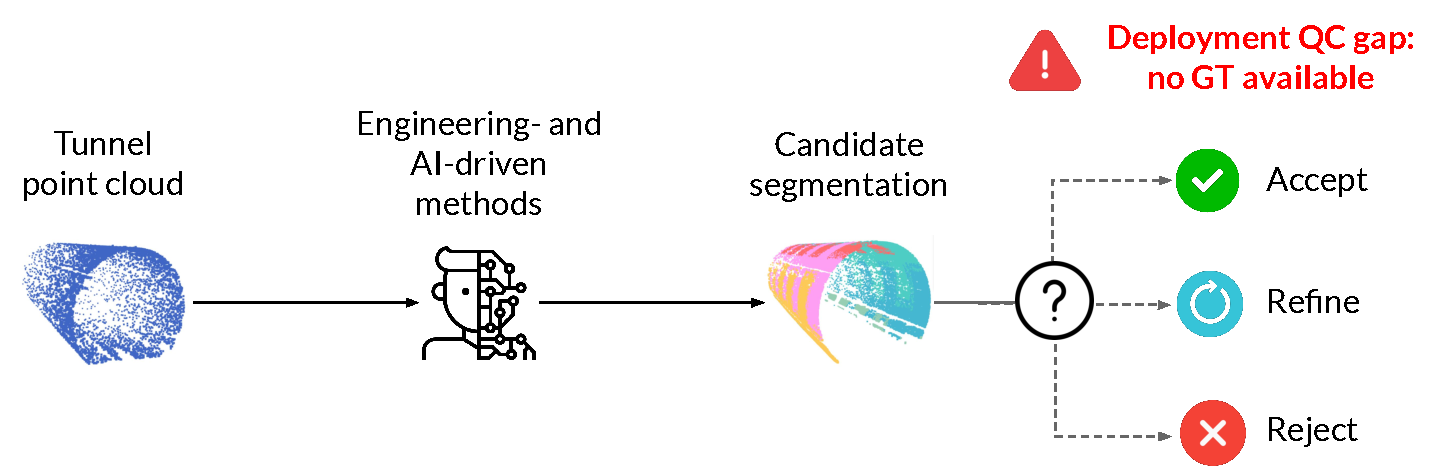
\includegraphics[width=0.8\textwidth]{figs/motivation.pdf}
\caption{Deployment quality-control (QC) problem: segmentation methods produce candidate outputs, but practitioners still need to decide whether to accept, refine, or flag each result without new GT labels.}
\label{fig:deployment_qc_gap}
\end{figure*}

\hl{This gap matters in practice for two reasons. First, an undetected segmentation failure propagates silently into every downstream measurement taken from it, so a fixed configuration that emits no quality signal shifts the burden of checking onto the engineer for every new scan. Second, re-tuning the pipeline for the new tunnel is blind under the same constraint: with no ground-truth (GT) labels, a parameter change cannot be confirmed as an improvement, and a search that maximises an unverified score can quietly make the output worse. Practitioners therefore need a deployment-time decision that requires no new labels: accept the output, refine it, or flag it for human review} (Fig.~\ref{fig:deployment_qc_gap}).

Previous studies show that segmentation accuracy can be estimated without GT labels for the new case. In medical imaging, for example, quality estimators learn from labelled development data or assess new outputs through labelled reference collections~\cite{valindria2017rca,robinson2018segmentationQuality,fournel2021segmentationQC}. However, it remains unclear how well these approaches transfer to tunnel point-cloud pipelines, where annotations are limited and processing often relies on geometry-dependent parameter settings. This motivates our central research question: \emph{Can intermediate tunnel-segmentation measurements support accuracy estimation and parameter self-refinement on unseen scans without new GT labels?}

We therefore propose Proxy4Tun, a QC framework that estimates segmentation accuracy from intermediate pipeline measurements and uses that estimate both to gate outputs and to guide self-refinement, without GT labels at deployment. Calibration requires one labelled subset and one expert reference per Seg2Tunnel lining family (staggered, continuous, and complex ring layouts). Preprocessing quality (PQ) describes the completeness and geometric plausibility of the segmentation input. Structure coherency (SC) describes agreement between predicted boundaries and detected joints, segmentation coverage, and consistency across rings. \hl{Within a pipeline adapted from SAM4Tun}~\cite{ye2025sam4tun}\hl{, bounded sampling across prescribed parameter ranges and uncertainty-guided Bayesian exploration produce 120 calibration runs spanning all three lining families; each run is scored against the development annotation for its corresponding family. We then run an ablation study over candidate PQ/SC feature sets and select a four-feature ridge-regression proxy; its coefficients are fitted on the calibration runs and then frozen, so that no held-out scan influences the estimator that judges it.} We hypothesise that the relationship between these measurements and segmentation accuracy generalises to unseen scans \textit{across lining families}. \hl{The frozen proxy is tested on 54 held-out runs from 27 subsets, each paired with a constructed degradation and gated at a pre-specified threshold of $0.4$. Self-refinement is then tested against a demanding baseline, the expert references themselves: under an identical three-attempt budget and the same proxy-based selection rule, proposals from three large language models (Fable-5.1, Gemini-3.8, GPT-5.6) are compared with adaptive-random proposals, so that the contribution of the proxy can be separated from the contribution of the proposer.}

\hl{The contributions of this paper are as follows:}
\begin{enumerate}
\item \hl{One labelled subset and one expert reference per lining family, expanded by bounded sampling and uncertainty-guided Bayesian exploration, suffice to fit a four-feature PQ/SC proxy that transfers to held-out scans (Spearman $\rho=0.791$), showing that intermediate tunnel-pipeline measurements carry accuracy information.}
\item \hl{The proxy is frozen and the $0.4$ threshold fixed before any held-out scoring, so the 27/27 reference--degradation rankings and 18/18 severe proposal failures test the gate rather than tune it, giving each new scan an accept, refine, or flag decision.}
\item \hl{Under identical starts, budget, and selection rule, LLM arms reach mean mIoU of $0.765$--$0.786$, compared with $0.750$ for adaptive-random, with $7$--$19\%$ harmful proposals versus $62\%$. Retrospective analysis shows that LLM refinement gains concentrate at lower initial accuracy, averaging $+0.077$ mIoU across six subsets with initial mIoU of $0.5$--$0.7$.}
\end{enumerate}

The rest of this paper is organised as follows. Section~\ref{sec:related} reviews related work. Section~\ref{sec:methods} presents the methodology and experimental design. Section~\ref{sec:results} reports the results, Section~\ref{sec:discussion} discusses findings and limitations, and Section~\ref{sec:conclusions} concludes.




\section{Related work}
\label{sec:related}

The review follows four connected questions: how segmentation methods adapt to changing conditions, how their outputs can be assessed without new GT labels, how calibration data can be obtained with limited annotations, and how assessment feedback can guide self-refinement.

\subsection{Tunnel segmentation and adaptation}

Methods for tunnel point-cloud segmentation range from geometric pipelines to supervised and foundation-model-based approaches. Engineer-designed pipelines use geometric rules and thresholds to identify lining surfaces and segment boundaries, but their settings may need adjustment when tunnel geometry, joint layout, or scan quality changes~\cite{huang2021bim,weidner2024generalized,wang2025automated}. PointNet++, RandLA-Net, Mask3D, and TD3D are general point-cloud neural networks that learn geometric representations from labelled 3D datasets~\cite{qi2017pointnet,hu2020randla,schult2023mask3d,kolodiazhnyi2024td3d}. Tunnel-specific supervised methods adapt these ideas with engineering constraints; LiningNet, for example, integrates structural geometry for lining segmentation~\cite{lin2025liningnet}. However, labelled tunnel data remain limited, and adapting supervised models to substantially different conditions may require additional annotations and retraining~\cite{su2024review, cha2024deep}.

Foundation-model pipelines reduce the need for task-specific training by using models pre-trained on large datasets. One practical approach is to project point clouds into two-dimensional images that can be processed by vision models. Prompt-based segmentation models include SAM~\cite{kirillov2023sam}, SAM2~\cite{ravi2024sam2}, and SEEM~\cite{zou2023segment}; infrastructure applications of such models include crack segmentation~\cite{ge2024cracksam,ye2024sam} and Scan-to-BIM workflows~\cite{wang2024omni,pan2024zero,ye2026maintenance}. For tunnel linings, SAM4Tun unfolds point clouds into panoramic images and generates template-based prompts for SAM to segment lining components without task-specific model training~\cite{ye2025sam4tun}. However, its preprocessing and prompting stages involve many interdependent parameters that encode assumptions about lining geometry and scanning conditions. When those conditions change, tuning these interdependent parameters can require substantial effort and domain expertise.

R4Tun addresses this parameter-adaptation problem by using a reference configuration, intermediate pipeline measurements, and engineering knowledge to guide LLM-proposed adjustments to SAM4Tun within prescribed parameter ranges~\cite{taoR4Tun}. Its adaptation proceeds without GT access, while the resulting segmentation accuracy is evaluated against GT offline. This supports the use of structured context to propose adjustments, but leaves a separate assessment task: \textit{determining the accuracy of the initial and adjusted outputs when new GT labels are unavailable}.

\subsection{Quality estimation without new GT labels}

Existing studies estimate segmentation quality from observable properties of the data and segmentation outputs. In medical imaging, Kohlberger et al. use segmentation features to predict overlap error and Dice scores~\cite{kohlberger2012evaluating}, while Robinson et al. learn to predict quality from image--segmentation pairs~\cite{robinson2018segmentationQuality}. For point clouds, LidarMetaSeg combines input features with network confidence measures to estimate the quality of connected semantic segments in self-driving scenes~\cite{colling2021lidarmetaseg}. Consistency between processing outputs can also provide evidence, although agreement does not guarantee correctness: different LiDAR processing streams can agree on an incorrect label~\cite{bogdoll2025labelfree}. These studies suggest that data properties and output consistency can help assess quality, provided their relationship with actual accuracy is established.

Reference-based approaches provide another source of assessment evidence. Reverse Classification Accuracy (RCA) treats a new segmentation as provisional labels, trains a reverse classifier, and evaluates that classifier on labelled reference images~\cite{valindria2017rca}. Its performance on those references is used to estimate the quality of the original segmentation. ConfIC-RCA further uses retrieval of relevant reference images and in-context reverse segmentation to estimate quality~\cite{cosarinsky2026conficrca}.

These studies motivate estimating accuracy from observable processing and segmentation features, avoiding the need for new GT labels at deployment. Proxy4Tun uses expert parameter configurations to generate calibration examples on a small labelled development set, then freezes the estimator and scores candidate outputs on new scans using only observable pipeline measurements. The remaining question is whether limited labelled tunnel data can support an estimator that remains useful on unseen scans and during parameter refinement across lining families.

\subsection{Calibration with limited labelled data}

Training a quality estimator requires examples spanning successful and degraded segmentations, but these examples need not require additional scan annotations. Robinson et al. generate multiple segmentations by varying model settings and reuse existing annotations to obtain quality targets~\cite{robinson2018segmentationQuality}. The same labelled input can therefore provide several examples of how processing choices affect accuracy. The challenge is to select useful settings without evaluating every possible combination.

Bayesian optimisation methods motivate incorporating prior knowledge when selecting which settings to evaluate. BOPrO encodes user beliefs about promising parameter regions, while $\pi$BO specifies a probability distribution over where the optimum is expected to lie~\cite{souza2020prior,hvarfner2022pibo}. Proxy4Tun does not implement these Bayesian optimisation mechanisms to locate an optimum. Instead, it uses Bayesian exploration: it starts with a space-filling design across the prescribed ranges~\cite{joe2008constructing}, fits a Gaussian-process surrogate to the observed accuracy response, and selects additional evaluations where predictive uncertainty is highest to broaden evidence across the parameter space~\cite{gramacy2009adaptive,gramacy2020surrogates}. The same development annotations are reused to calculate GT mIoU for each run.

\subsection{Feedback-guided self-refinement}

LLM-based agents can revise results by proposing changes, evaluating their effects, and using feedback to guide subsequent attempts. Self-Refine asks the model to critique and revise its output, while Reflexion records lessons from task feedback for later attempts~\cite{madaan2023selfrefine,shinn2023reflexion}. AlphaEvolve and the Darwin G\"odel Machine extend feedback-guided search to modifying programs or agent code using automated evaluation~\cite{novikov2025alphaevolve,zhang2025darwin}. However, repeated revision does not guarantee improvement. Self-correction without external feedback can fail, and increasing an imperfect proxy score can reduce performance when assessed separately~\cite{huang2024selfcorrect,gao2023overoptimization}.

Feedback can also provide diagnostic information to guide subsequent proposals. ReAct demonstrates how observations from the environment can inform subsequent actions~\cite{yao2023react}. In Proxy4Tun, PQ and SC measurements provide this feedback context for LLM reasoning: an incomplete depth map or disagreement between detected joints and predicted boundaries can indicate which stages warrant inspection.

We use a linear proxy to expose how each measurement contributes to the predicted score, supporting interpretation of the estimate~\cite{rudin2019stop}. Proxy4Tun then examines whether this frozen proxy can guide bounded parameter self-refinement via LLM proposals.

% ══════════════════════════════════════════════════════════════════════════
\section{Methodology}
\label{sec:methods}

Proxy4Tun has two phases: (i) development-time calibration on labelled scans to learn a proxy from PQ/SC measurements, and (ii) deployment-time scoring and bounded self-refinement on new scans without GT labels. \hl{Four requirements of that setting shape the design, each met by one choice:}
\begin{enumerate}
\renewcommand{\labelenumi}{\roman{enumi}.}
\item \textbf{Scarce labels.} Calibration uses one labelled subset and one expert reference per family.
\item \textbf{Transfer.} The proxy is selected by leave-one-family-out (LOFO) cross-validation performance and then frozen.
\item \textbf{Auditability.} A compact linear proxy exposes how each measurement contributes to the score.
\item \textbf{Attribution.} Self-refinement compares LLM proposals with a random control under the same budget and the same selection rule.
\end{enumerate}
Sections~\ref{sec:problem-def}--\ref{sec:agent-design} describe the task, calibration, and self-refinement; Section~\ref{sec:exp-setup} the evaluation.

\begin{figure*}[t]
\centering
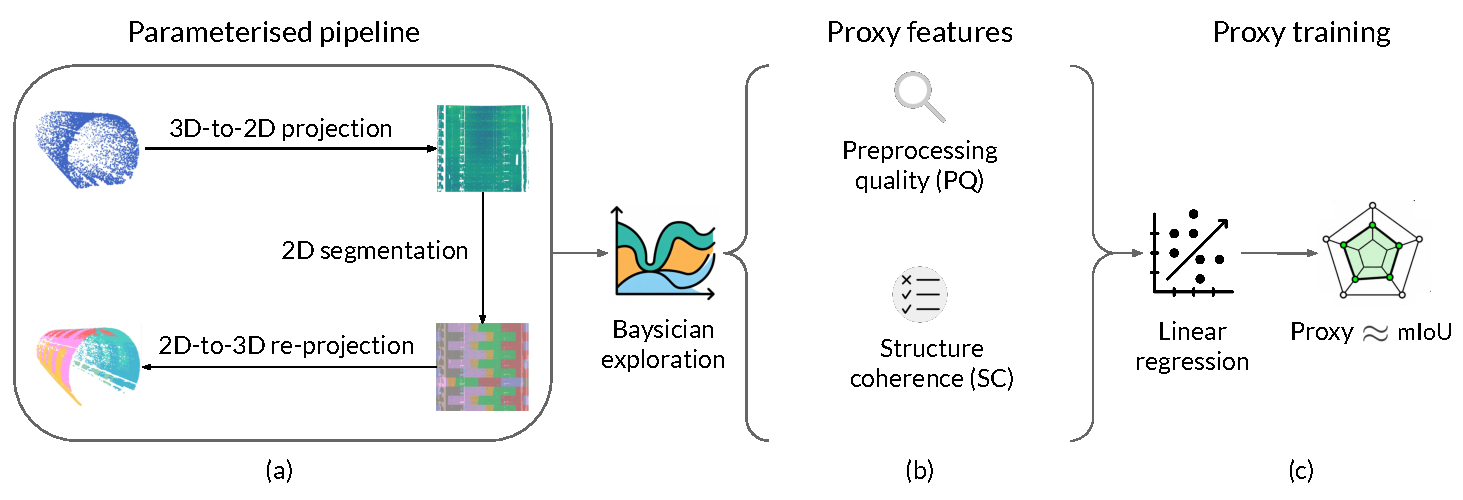
\includegraphics[width=\textwidth]{figs/intrinsics.pdf}
\caption{Development and use of the accuracy proxy. Parameter variations generate segmentation outputs with different accuracies. PQ and SC measurements from each run are paired with GT mIoU to train the proxy. Once fitted, the proxy estimates accuracy on new runs using measurements available without GT. The score is an estimate of segmentation accuracy, not a guarantee of correctness.}
\label{fig:intrinsic_proxy_scoring}
\end{figure*}


\subsection{Task definition}
\label{sec:problem-def}

Given a raw point cloud of a tunnel section, the task is to assign each point a structural label: background, key segment (K), adjacent segments (B), and standard segments (A). Seg2Tunnel, the benchmark dataset we use, groups linings into three families (staggered, continuous, and complex). These families differ in ring geometry and acquisition conditions and, most critically for our task, in the key-block (K) layout: ring-to-ring repeating, fixed ring-wise order, and no repeating pattern (Fig.~\ref{fig:task}). 

Given a completed run, Proxy4Tun estimates its mIoU from intermediate outputs alone, so the score can be compared across runs of the same scan under different parameters. No GT for the new scan is used at any point of scoring or self-refinement.

\begin{figure*}[t]
\centering
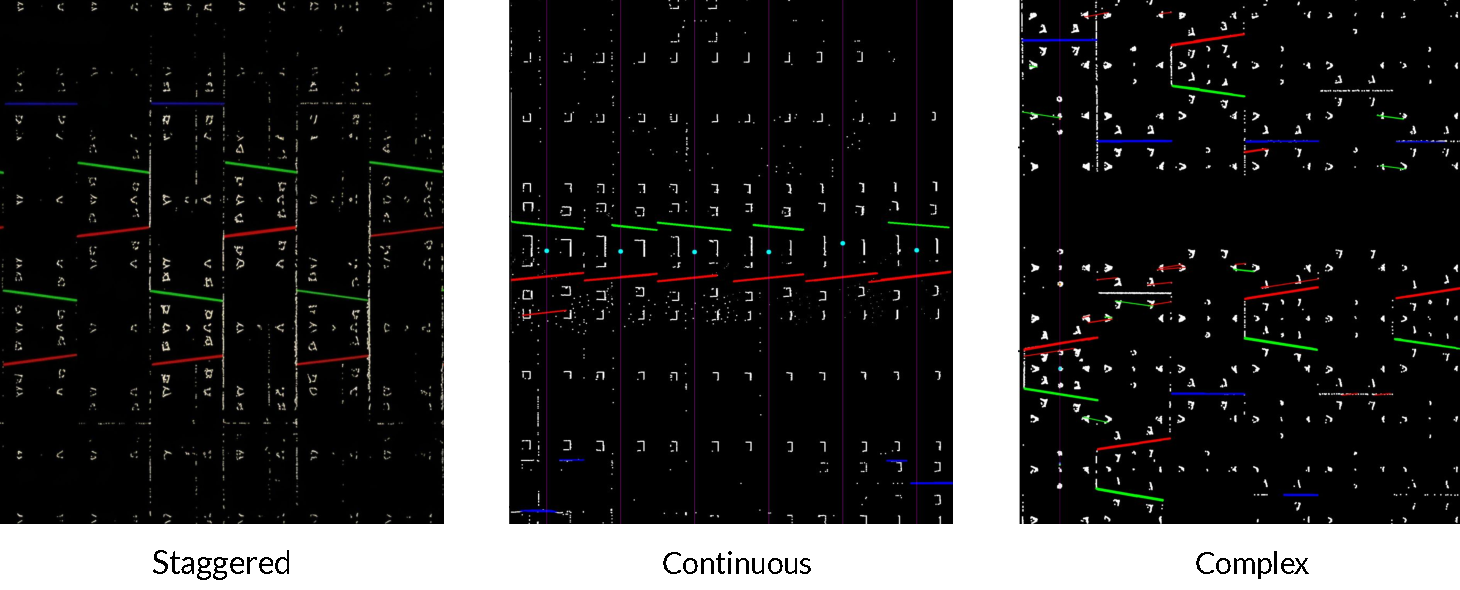
\includegraphics[width=0.8\textwidth]{figs/task.pdf}
\caption{Tunnel-lining block types: key block (K), adjacent block (B), and standard block (A), with background labelled separately. A ring contains six or seven individual lining blocks depending on its family.} 
\label{fig:task}
\end{figure*}




\subsection{Framework overview}
\label{sec:method}

The framework links a parameterised segmentation pipeline, an offline procedure for learning the mIoU proxy, and a deployment-time self-refinement loop that compares candidates using the frozen proxy (Fig.~\ref{fig:intrinsic_proxy_scoring}). Throughout, the stage algorithms are fixed and only their parameters vary. 


\subsubsection{Segmentation pipeline}
\label{sec:pipeline}

The pipeline is adapted from SAM4Tun~\cite{ye2025sam4tun} for the three Seg2Tunnel lining families~\cite{lin2024seg2tunnel}. Figure~\ref{fig:pipeline} illustrates the processing stages.

\begin{figure*}[t]
\centering
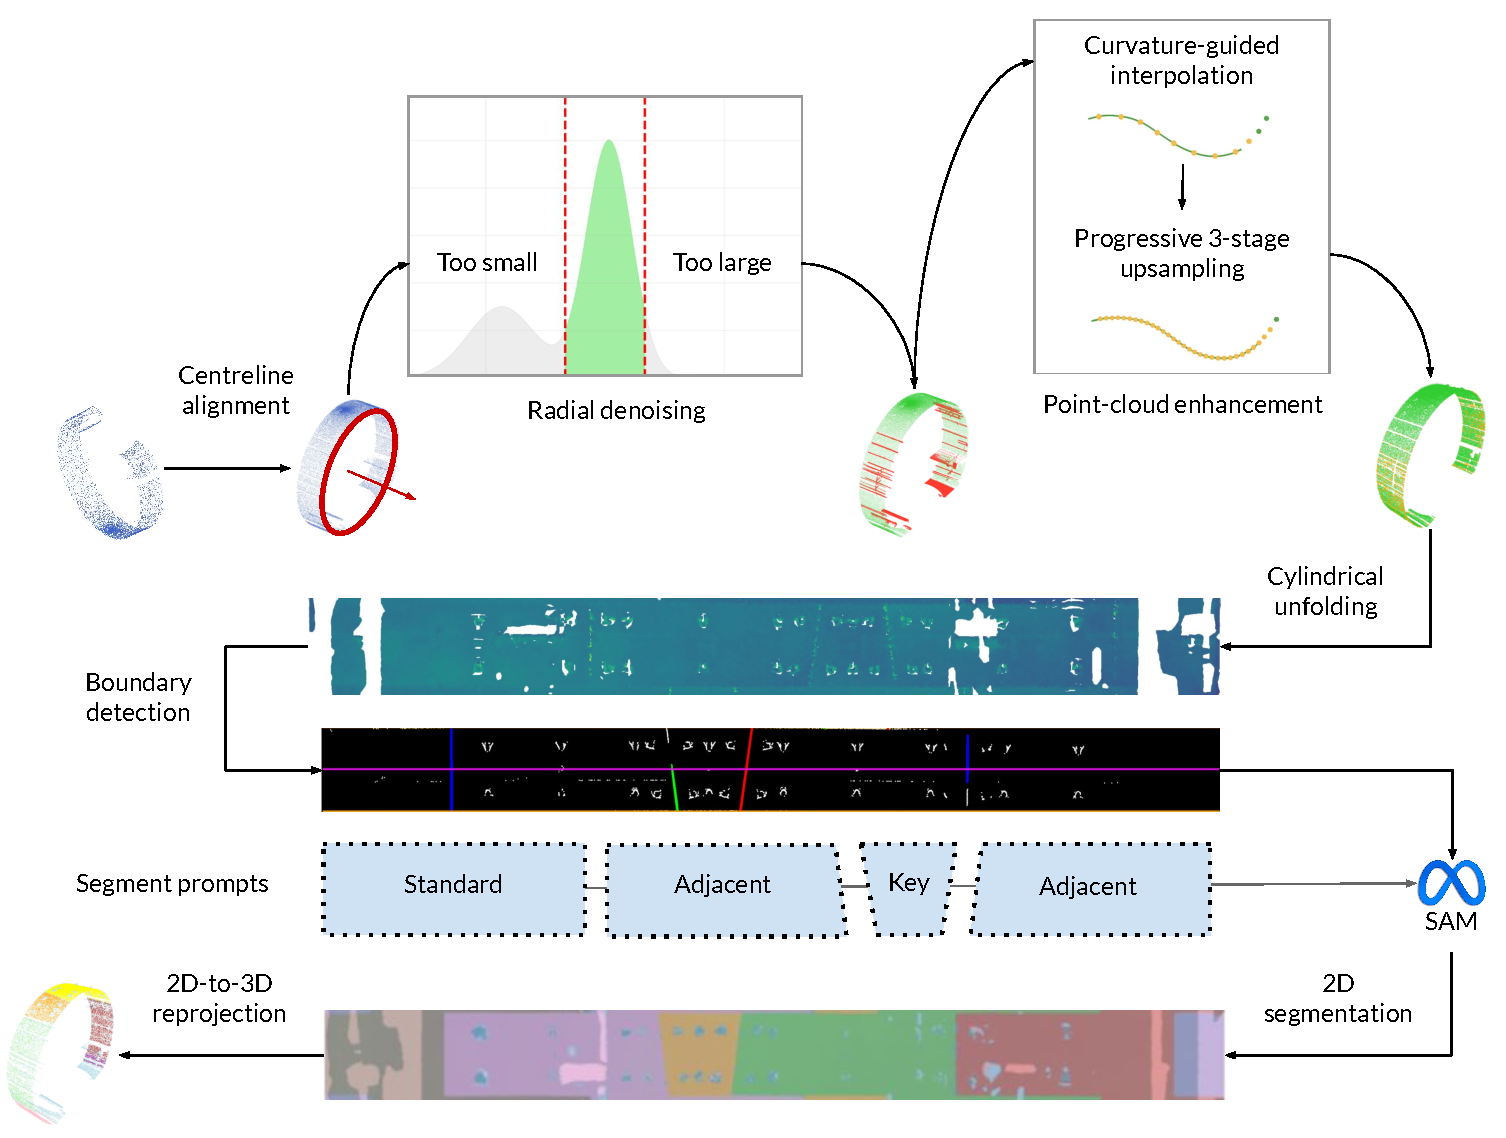
\includegraphics[width=0.98\textwidth]{figs/pipeline.pdf}
\caption{Segmentation pipeline adapted from SAM4Tun. Geometric alignment, filtering, and enhancement produce a depth representation for boundary detection and template-based SAM prompting. The resulting masks are reprojected onto the point cloud. Intermediate outputs provide PQ and SC measurements. The stage algorithms remain fixed; exploration and self-refinement adjust their parameters.}
\label{fig:pipeline}
\end{figure*}

\begin{enumerate}
\item \textbf{Unfolding.}
RANSAC-based cross-sectional ellipse fitting and centreline estimation establish a cylindrical coordinate system~\cite{fischler1981ransac}. The lining surface is represented panoramically, with depth describing radial distance from the centreline. Coordinate orientation is fixed so that block positions retain the same meaning across runs.

\item \textbf{Denoising.}
Radial masks and grid-based point-density filtering remove points inconsistent with the expected lining surface. The filtering follows the density-based principle underlying DBSCAN~\cite{ester1996dbscan}. Its settings affect both unwanted-point removal and the amount of lining data retained.

\item \textbf{Enhancement.}
Curvature-guided interpolation and progressive upsampling improve the completeness of the depth representation before detection, while preserving joint boundaries.

\item \textbf{Boundary detection.}
Orientation-specific Hough transforms identify candidate ring and block boundaries~\cite{duda1972hough}. These detections are organised according to the expected family layout.

\item \textbf{Segmentation and reprojection.}
The detected layout defines template-based prompts for SAM~\cite{kirillov2023sam}. The resulting image masks are mapped back to the point cloud to obtain three-dimensional block labels.
\end{enumerate}

Each family has an expert-tuned \emph{family reference}: a complete parameter configuration that serves as the starting point for calibration and self-refinement. A candidate update lists only the parameters to change and is applied to an explicitly recorded base configuration. Unchanged parameters retain their base values. Appendix~\ref{app:anchor-parameter} lists the expert family references, and Appendix~\ref{app:search-bounds} provides the exploration bounds.


\subsubsection{Generating calibration examples}
\label{sec:bo-experience}

\hl{With the pipeline and its family references fixed, the next step is to learn how its intermediate measurements relate to accuracy.} Calibration requires examples linking observable pipeline measurements
to segmentation accuracy under successful and degraded parameter
settings. We generate these examples by perturbing the expert family reference on a single labelled development subset per family.

Two sampling stages balance coverage and informativeness. First, scrambled-Sobol sampling
provides 32 valid trials spread across the prescribed parameter
ranges~\cite{joe2008constructing}, so that common failure modes (over-filtering, missed joints, wrong ring count) appear alongside near-reference runs. Second, Bayesian exploration adds eight valid trials where a Gaussian-process (GP) model of GT mIoU is most uncertain~\cite{gramacy2009adaptive,gramacy2020surrogates}. We explore uncertainty rather than maximise accuracy because the proxy must rank good and bad runs, which needs evidence across the response rather than a single optimum (Appendix~\ref{app:bo-config}).

Each family contributes 40 valid runs, giving 120 runs across the
three families. Each
valid run records its parameter setting, PQ and SC measurements,
and GT mIoU. Algorithm~\ref{alg:bo_exploration} and Figure~\ref{fig:b-p} summarise the procedure; Appendix~\ref{app:search-bounds} lists the parameter bounds.

\begin{figure*}[t]
\centering
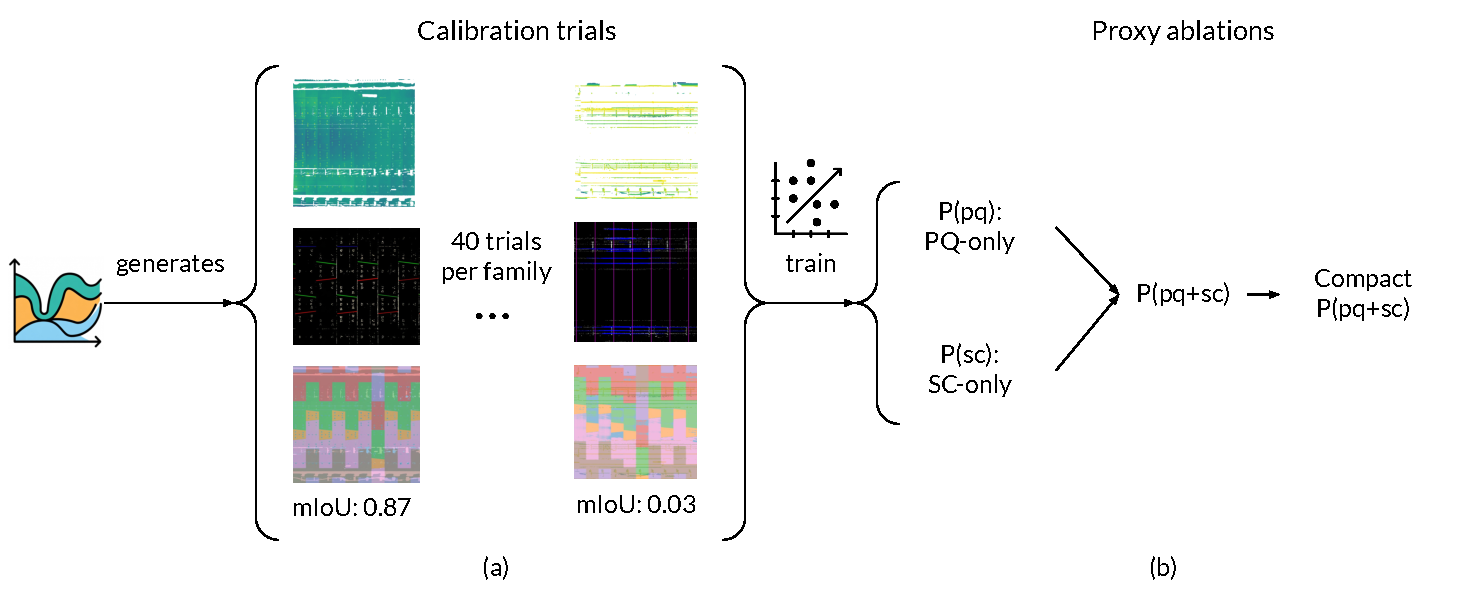
\includegraphics[width=\textwidth]{figs/b-p.pdf}
\caption{Calibration-example generation and feature comparison.
(a) Each lining family contributes 32 valid scrambled-Sobol trials
and eight valid Bayesian exploration trials selected by GP
uncertainty. All trials reuse the same development-subset annotations.
(b) The resulting measurements and GT mIoU values support comparison
of PQ-only, SC-only, combined, and compact combined feature sets
for the accuracy proxy.}
\label{fig:b-p}
\end{figure*}

\begin{algorithm}[ht]
\caption{Generating calibration examples through space-filling
sampling and Bayesian exploration}
\label{alg:bo_exploration}
\begin{algorithmic}[1]
\Require Development subset $D_f$ with GT annotations $Y_f$
\Require Reference configuration $P_f^{\mathrm{ref}}$; expected ring count $N_{\mathrm{exp}}=10$
\Require Parameter bounds $\Theta_f$;
         valid-trial budgets $N_0=32$, $N_1=8$;
         candidate-pool size $M=2048$
\Ensure Calibration records $\mathcal{T}_f$
\State $\mathcal{T}_f\gets\emptyset$;
       $n_0\gets0$; $n_1\gets0$
\State Initialise a scrambled-Sobol sequence
\Statex \textit{Phase 1: broad initial coverage}
\While{$n_0<N_0$}
    \State Draw the next Sobol point and map it to
           permitted parameter values $\theta\in\Theta_f$
    \State $P\gets\operatorname{Apply}
           (P_f^{\mathrm{ref}},\theta)$
    \State $R\gets\operatorname{Pipeline}(D_f,P)$
    \If{$R$ is valid and required measurements are available}
        \State $\mathbf{x}\gets\operatorname{Features}(R,N_{\mathrm{exp}})$
        \State $y\gets\operatorname{mIoU}(R,Y_f)$
        \State Append $(\theta,\mathbf{x},y)$
               to $\mathcal{T}_f$
        \State $n_0\gets n_0+1$
    \Else
        \State Log the failed or incomplete trial
    \EndIf
\EndWhile
\Statex \textit{Phase 2: Bayesian exploration}
\State Fit GP to the $(\theta,y)$ pairs in $\mathcal{T}_f$
\While{$n_1<N_1$}
    \State Draw $M$ random candidate settings
           $\mathcal{P}_t$ within $\Theta_f$
    \State $\theta\gets
           \arg\max_{\vartheta\in\mathcal{P}_t}
           \sigma_t(\vartheta)$
    \State $P\gets\operatorname{Apply}
           (P_f^{\mathrm{ref}},\theta)$
    \State $R\gets\operatorname{Pipeline}(D_f,P)$
    \If{$R$ is valid and required measurements are available}
        \State $\mathbf{x}\gets\operatorname{Features}(R,N_{\mathrm{exp}})$
        \State $y\gets\operatorname{mIoU}(R,Y_f)$
        \State Append $(\theta,\mathbf{x},y)$
               to $\mathcal{T}_f$
        \State Update GP using the expanded $\mathcal{T}_f$
        \State $n_1\gets n_1+1$
    \Else
        \State Log the failed or incomplete trial
    \EndIf
\EndWhile
\State \Return $\mathcal{T}_f$
\end{algorithmic}
\end{algorithm}

\subsubsection{PQ and SC measurements}
\label{sec:features}

Measurements form two groups because failures arise in two places: upstream, where the depth representation may be incomplete or misaligned (PQ), and downstream, where the recovered layout may be incoherent even when the input is sound (SC). Table~\ref{tab:candidate-features} lists the ten candidates (four PQ, six SC), all computed without GT. The only external input is the expected ring count $N_{\mathrm{exp}}$, which is known from design or scan records; comparing it with the detected count flags a mis-recovered layout. SC is particularly useful for the complex family because it does not assume a fixed keystone pattern. However, high SC does not guarantee correctness: because joint detections also drive SAM prompting, joint--boundary agreement can share correlated errors with the segmentation. It is evidence, not proof, of correctness.

\begin{table*}[t]
\caption{Candidate measurements for the mIoU accuracy proxy (four PQ, six SC). Pixel quantities refer to the 5\,mm depth-image grid. The four retained by the frozen proxy are marked $\star$. Stages: 1---unfolding; 2---denoising; 3---enhancement; 4---joint detection; 5---SAM segmentation. Combined indices indicate measurements using outputs from both stages.}
\label{tab:candidate-features}
\centering
\small
\setlength{\tabcolsep}{3pt}
\begin{tabular}{p{0.05\textwidth} p{0.27\textwidth} p{0.45\textwidth} p{0.16\textwidth}}
\toprule
Group & Measurement & Meaning & Stage \\
\midrule
PQ & Unfolding fit residual & Centreline fit error & 1 \\
 & Orientation agreement & Difference between inferred and expected axes & 1 \\
 & Point retention & Fraction of input points kept after denoising & 2 \\
 & Missing-depth rate $\star$ & Fraction of depth-image pixels without depth after enhancement & 3 \\
SC & Ring-count residual $\star$ & $|N_{\mathrm{det}}-N_{\mathrm{exp}}|$ against the design/acquisition prior & 4 \\
 & Edge support & Fraction of label-boundary pixels within 25\,px of a depth edge & 3+5 \\
 & Correspondence score $\star$ & F1 between detected joint lines and predicted block boundaries at 15\,px & 4+5 \\
 & Line--boundary distance & Symmetric mean distance (capped at 200\,px) between joints and boundaries & 4+5 \\
 & Fill rate $\star$ & Fraction of input points assigned a non-background label & 5 \\
 & Phase incoherence & Inconsistency of label ordering across rings & 5 \\
\bottomrule
\end{tabular}
\end{table*}

\subsubsection{Learning the accuracy proxy}
\label{sec:ridge-proxy}

The proxy maps these PQ and SC measurements to an estimated mIoU. We use Ridge regression to obtain a compact linear proxy that serves as an explicit scoring rule. Regularisation stabilises estimation under correlated predictors~\cite{hoerl1970ridge,pedregosa2011sklearn}, and the linear form makes each measurement's contribution directly interpretable, enabling inspection of the feedback used in LLM-guided refinement. We use this form for transparency and do not claim superiority over nonlinear alternatives.

For a feature vector $\mathbf{x}\in\mathbb{R}^{d}$, the prediction is
\begin{equation}
\hat{y}(\mathbf{x})
=
b+\sum_{j=1}^{d}
w_j\frac{x_j-\mu_j}{s_j},
\label{eq:ridge-proxy}
\end{equation}
where $\mu_j$ and $s_j$ are the mean and standard deviation estimated on the training data, $w_j$ is the fitted coefficient, and $b$ is the intercept. Coefficients are fitted by least squares with an $\ell_2$ penalty whose strength $\alpha$ is selected using only the training data.

We compare PQ-only, SC-only, combined, and compact combined models (Table~\ref{tab:proxy-ablation}). The notation $P(q)$ denotes the PQ-only model, $P(c)$ denotes the SC-only model, and $P(q{+}c)$ denotes their combination.

\begin{table}[ht]
\caption{Proxy feature and model comparisons.}
\label{tab:proxy-ablation}
\centering
\begin{tabular}{p{0.38\columnwidth} p{0.52\columnwidth}}
\toprule
Model & Definition \\
\midrule
$P(q)$ & Four PQ features \\
$P(c)$ & Six SC features \\
$P(q{+}c)$ & All ten candidate features \\
Compact $P(q{+}c)$ & Four selected features; one pooled model \\
Compact per-family & The same four features; one model per family \\
\bottomrule
\end{tabular}
\end{table}

LOFO validation fits each model on two families and tests it on the third; feature selection and $\alpha$ are tuned inside each fold, never on the held-out family. The compact set keeps the four measurements (\hl{one PQ, three SC}) that transfer best across folds; it is not tuned to maximise every development metric. The final pooled model is then fitted on all 120 calibration runs and frozen.

The proxy score provides a common basis for comparing outputs. Regression coefficients describe fitted associations with accuracy; they are not causal prescriptions for parameter changes. Algorithm~\ref{alg:proxy} separates model development from deployment scoring.

\begin{algorithm}[ht]
\caption{Proxy calibration and deployment scoring}
\label{alg:proxy}
\begin{algorithmic}[1]
\Require Calibration records $\mathcal{T}=\bigcup_f\mathcal{T}_f$; candidate feature sets
\Require Fixed extraction conventions, including $N_{\mathrm{exp}}=10$
\Ensure Frozen proxy package $g$
\For{each candidate feature set $V$}
    \For{each held-out family $f$}
        \State Use the other two families as training data
        \State Fit feature scaling and select $\alpha$ within the training data
        \State Fit the model and predict the held-out family's mIoU
    \EndFor
    \State Record training and LOFO prediction metrics
\EndFor
\State Select the compact four-feature set by LOFO Spearman, retaining PQ and SC
\State Fit pooled scaling and Ridge regression on all 120 calibration records
\State Freeze feature definitions, order, scaler, coefficients, and intercept
\Statex
\State Receive a new completed run $r$
\State $\mathbf{x}\gets\operatorname{Features}(r,N_{\mathrm{exp}})$ in the frozen feature order
\State $\hat{y}\gets g(\mathbf{x})$
\State \Return $\hat{y}$
\end{algorithmic}
\end{algorithm}


\subsection{Proxy-guided parameter self-refinement}
\label{sec:agent-design}

The proxy estimates accuracy but does not decide which parameters to change. An LLM agent (GPT-5.6, Gemini-3.8, and Claude Fable-5.1) proposes the change (Fig.~\ref{fig:agent}). It sees the family reference, the current run's intermediate outputs and PQ/SC measurements, the proxy score, and short engineering notes linking observable symptoms to likely adjustments (Appendices~\ref{app:ontology} and~\ref{app:prompt}). It returns one bounded parameter update with a brief rationale.

Three protocol choices define the process:
\begin{enumerate}
\renewcommand{\labelenumi}{\roman{enumi}.}
\item \textbf{Start.} Each case begins from its expert family reference rather than a weak configuration, so improvement must beat what a practitioner would already deploy.
\item \textbf{Budget.} Three attempts per case without early stopping give every arm the same number of executions and hold cost to roughly 15 GPU-minutes per case.
\item \textbf{Control.} The random arm shares bounds, budget, and selection rule, so it isolates whether the use of pipeline evidence, rather than search itself, produces gains.
\end{enumerate}

\begin{figure*}[t]
\centering
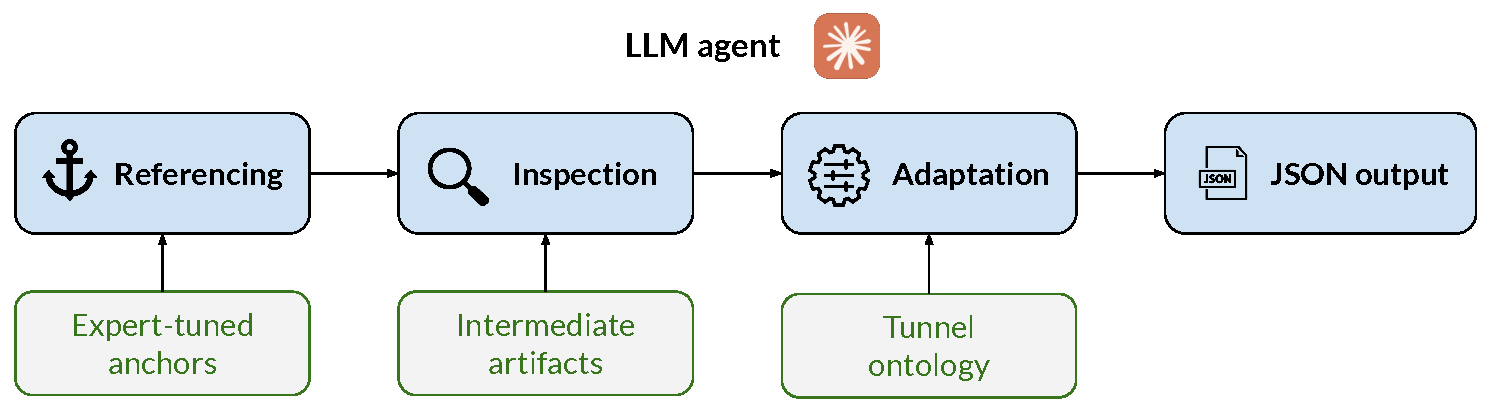
\includegraphics[width=0.8\textwidth]{figs/agent.pdf}
\caption{LLM-guided parameter proposals. The agent compares the current run with engineering references, inspects intermediate outputs and PQ/SC measurements, and returns a bounded parameter update with a rationale. After execution, the frozen proxy scores the candidate. Candidate retention depends only on the proxy score.}
\label{fig:agent}
\end{figure*}

Each attempt has three steps:
\begin{enumerate}
\item \textbf{Propose.}
The agent names a likely failure mode from the evidence and returns a small update with a one-line rationale.

\item \textbf{Run.}
The update is checked against allowed names and ranges; if valid, the pipeline is re-run and PQ/SC recomputed. An invalid or failed attempt still uses one of the three slots.

\item \textbf{Score.}
The frozen proxy scores the new run; update, score, and outcome are stored as feedback for the next attempt.
\end{enumerate}

\textbf{Random search (control).}
The random arm changes a similar number of parameters to the LLMs, but picks which ones and what values at random inside the same bounds (Appendix~\ref{app:random-search}).
Unlike LLM updates, the random method does not read intermediate measurements.
Accepted random changes are applied on top of the current best configuration.

\textbf{Selection rule.} A new run replaces the current best only if its proxy score is more than $0.01$ higher (the \emph{retention margin}); smaller gains are within proxy noise and the earlier output is kept. Algorithm~\ref{alg:reflective_adaptation} summarises the loop shared by all arms.

\begin{algorithm}[ht]
\caption{Proxy-guided parameter self-refinement}
\label{alg:reflective_adaptation}
\begin{algorithmic}[1]
\Require Held-out scan; expert reference start; frozen proxy; budget of three attempts
\Ensure Best configuration kept after three attempts
\State Run the expert reference and score it with the proxy; keep it as the current best
\For{attempt $=1,2,3$}
    \State Propose one bounded update (LLM from evidence, or random)
    \State If the update is valid, re-run the pipeline and score the new output
    \State Keep the new output only if its proxy score exceeds the current best by more than $0.01$
\EndFor
\State \Return the kept configuration and its proxy score
\end{algorithmic}
\end{algorithm}


\subsection{Experimental setup}
\label{sec:exp-setup}
The evaluation addresses three questions: whether PQ and SC support accuracy estimation, whether the frozen proxy distinguishes reference outputs from controlled degradations on unseen scans, and whether proxy-guided self-refinement improves the 27 expert references. Each test is designed so that the proxy never sees GT for the scan it is judging. We use Seg2Tunnel subsets spanning staggered, continuous, and complex lining families~\cite{lin2024seg2tunnel}. One development subset per family (2-1, 3-1, 5-1) supplies the calibration runs; the other 27 subsets, nine per family, form the held-out panel (Table~\ref{tab:dataset}). Held-out GT is used only to report offline accuracy after the fact.\label{sec:dataset}

\begin{table*}[t]
\caption{Development and held-out subsets. One labelled development subset per family supplies the calibration trials; nine other subsets per family form the held-out panel.}
\label{tab:dataset}
\centering
\begin{tabular}{p{0.22\textwidth} p{0.24\textwidth} p{0.22\textwidth} p{0.22\textwidth}}
\toprule
Property & Staggered (T1, T2) & Continuous (T3) & Complex (T4, T5) \\
\midrule
Inner diameter & 5.5\,m & 5.9\,m & 7.5\,m \\
Ring length & 1.2\,m & 1.2\,m & 1.8\,m \\
Blocks per ring & 6 & 6 & 7 \\
Key-block layout & Ring-to-ring repeating pattern & Fixed ring-wise order & No repeating pattern \\
Scanning & Single-station & Multi-station & Single-station, offset \\
Development subset & 2-1 & 3-1 & 5-1 \\
Calibration runs & 40 & 40 & 40 \\
Held-out subsets & 1-1--1-5; 2-2--2-5 & 3-2--3-10 & 4-1--4-5; 5-2--5-5 \\
\bottomrule
\end{tabular}
\end{table*}


\subsubsection{Feature and model comparisons}
\label{sec:comparators}

Three development-time checks use the 120 calibration runs only:
\begin{enumerate}
  \item The feature-set comparison in Table~\ref{tab:proxy-ablation} reports training fit and LOFO transfer separately, because a model can fit its own families well and still fail on a new one.
  \item The pooled compact proxy is compared with three family-specific proxies (same four features, 40 runs each) to test whether one shared model costs accuracy relative to per-family fitting.
  \item A permutation control shuffles GT mIoU among runs within each family and refits 20 times; if the real-label LOFO correlation is not clearly above the shuffled ones, the features are only tracking family identity rather than accuracy.
\end{enumerate}
The frozen proxy is then tested once on the 27 unseen subsets.


\subsubsection{Paired degradation test}
\label{sec:stress-test}

The goal of the degradation set is to give a simple, controlled way to check whether the frozen proxy can tell \emph{better} outputs from \emph{worse} ones on unseen subsets. For each held-out subset we start from its family-reference output and then apply a small, pre-defined degradation (chosen from development-time experience and fixed before any held-out scoring), yielding 54 scored runs in total.

This paired setup avoids relying on rare, unlabelled natural failures and keeps the comparison fair: both outputs come from the same scan, so differences in difficulty across scans do not drive the result. The proxy scores both outputs, while GT mIoU is computed separately to verify that the degraded output is indeed worse. We then test whether the proxy ranks the reference above its degraded partner and whether a fixed threshold of $0.4$ flags the degraded output. Because the degradations are constructed, the result speaks to discrimination under these specific perturbations rather than reliability on naturally occurring failures.


\subsubsection{Self-refinement panel against family-specific references}
\label{sec:poc-protocol}

We test whether label-free self-refinement can improve already-strong family-specific references. For each held-out subset we start from its family reference (mean mIoU of $0.762$ across the 27-subset panel) and allow up to three refinement attempts.

Each subset is evaluated under four proposal arms---Fable-5.1, Gemini-3.8, GPT-5.6, and random search---all sharing the same frozen proxy, parameter bounds, budget, and selection rule (Algorithm~\ref{alg:reflective_adaptation}; Fig.~\ref{fig:verification}). Proposals and selection never see GT; GT is used only for offline reporting.

\begin{figure*}[t]
\centering
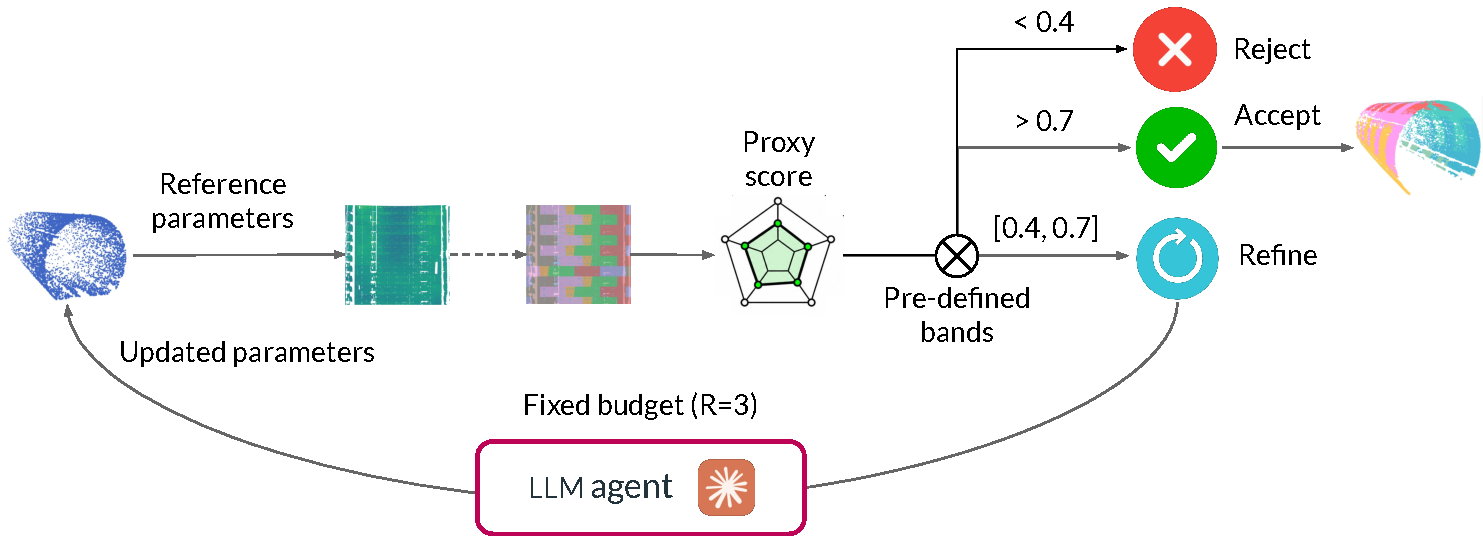
\includegraphics[width=0.9\textwidth]{figs/verification.pdf}
\caption{Self-refinement protocol shared by all arms. Each of the 27 family references receives three attempts; failed attempts consume budget and leave the kept configuration unchanged. A candidate replaces it only if its proxy score is more than $0.01$ higher. }
\label{fig:verification}
\end{figure*}

Table~\ref{tab:poc-config} summarises the shared protocol. Every proposed update (and, for LLM arms, its rationale), outcome, and score is logged; runs use a single NVIDIA RTX~5060 GPU.

\begin{table}[ht]
\caption{Self-refinement study configuration.}
\label{tab:poc-config}
\centering
\begin{tabular}{p{0.35\columnwidth} p{0.55\columnwidth}}
\toprule
Setting & Value \\
\midrule
Proposal arms & Fable-5.1; Gemini-3.8; GPT-5.6; random search \\
Starting configuration & Family-specific reference (per subset) \\
Panel & All 27 held-out reference starts \\
Context (LLM arms) & Engineering knowledge, outputs, PQ/SC measurements, proxy scores \\
Budget & Three proposal attempts per subset and arm \\
Early stopping & None \\
Output & Structured parameter update (and rationale for LLM arms) \\
Failure handling & Consumes one attempt; kept configuration unchanged \\
Selection & Proxy score only; replace the kept output if $>0.01$ higher (retention margin) \\
\bottomrule
\end{tabular}
\end{table}

Overall, the panel tests whether the proxy alone can drive improvements from strong starting points. It does not estimate success rates on an unfiltered deployment population, nor demonstrate sustained self-improvement beyond three attempts.


\subsubsection{Evaluation metrics}
\label{sec:metrics}

Offline segmentation accuracy is measured by mIoU. For evaluated block class $c$,
\begin{equation}
\operatorname{IoU}_c
=
\frac{\operatorname{TP}_c}
{\operatorname{TP}_c+\operatorname{FP}_c+\operatorname{FN}_c},
\qquad
\operatorname{mIoU}
=
\frac{1}{C}\sum_{c=1}^{C}\operatorname{IoU}_c,
\end{equation}
where $C=6$ for staggered and continuous rings and $C=7$ for complex rings.

We report results in three complementary views. First, we assess whether a proxy induces the \emph{same ordering} of candidates as ground-truth accuracy (Spearman $\rho$, since selection is ordinal), and we quantify the typical gap between proxy scores and true accuracy (mean absolute error, MAE); bootstrap 95\% confidence intervals indicate uncertainty. Second, in a paired reference vs.~degraded test, we report how often the proxy assigns a higher score to the reference (ties count as failures) and how reliably it flags the degraded output using a fixed decision threshold of $0.4$. Third, for self-refinement, we report (for each case) the score and accuracy before and after selection, making clear when selection improves or degrades true accuracy; confidence intervals again account for shared conditions within the same tunnel by resampling parent tunnels rather than subsets.

% ══════════════════════════════════════════════════════════════════════════
% ══════════════════════════════════════════════════════════════════════════
\section{Results}\label{sec:results}
% ══════════════════════════════════════════════════════════════════════════

The results follow the three questions of Section~\ref{sec:exp-setup}: whether PQ and SC carry accuracy information that transfers across families, whether the frozen proxy separates references from degradations on unseen scans, and whether it can guide improvement of already-strong references. A residual error analysis then shows where the four features stop seeing.

\subsection{Proxy calibration and feature ablation}
\label{sec:main-results}
\label{sec:proxy-ablation-results}

The selected proxy contains three SC measurements (correspondence F1@15, segmentation fill rate, and ring-count error) and one PQ measurement ( depth-map missing-pixel fraction). With training-standardised inputs, its fitted equation is
\begin{equation}
\begin{aligned}
\hat{y}={}&0.359+0.0872z_{\mathrm{corr}}+0.0939z_{\mathrm{fill}}\\
&-0.0386z_{\mathrm{ringerr}}-0.0545z_{\mathrm{nan}}.
\end{aligned}
\label{eq:four-proxy}
\end{equation}
Here, $z_{\mathrm{corr}}$ is correspondence F1@15, $z_{\mathrm{fill}}$ is fill rate, $z_{\mathrm{ringerr}}$ is ring-count error, and $z_{\mathrm{nan}}$ is missing-depth rate after standardisation. RidgeCV selects $\alpha=10.0$. These are conditional associations in a correlated linear model, not independent causal effects.

\begin{figure*}[t]
  \centering
  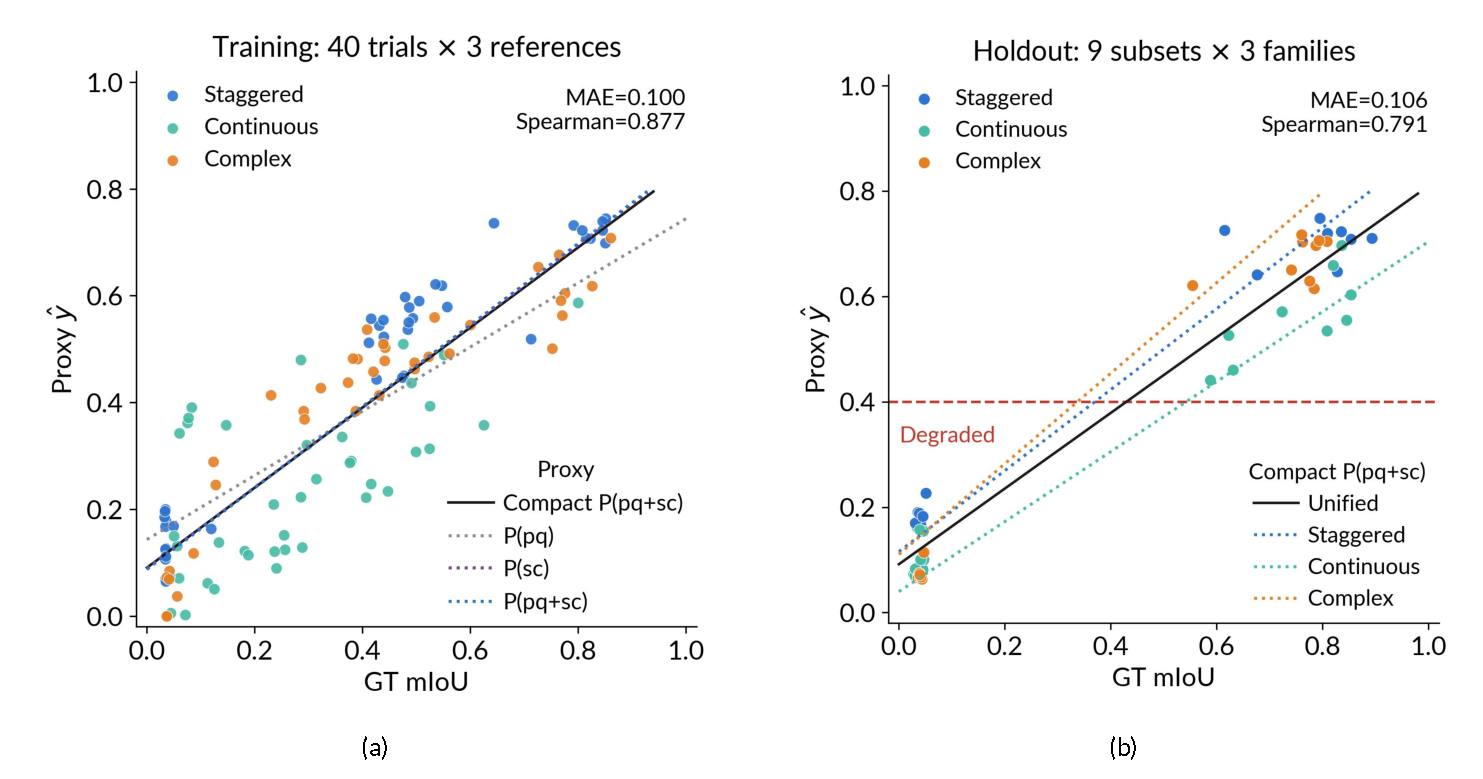
\includegraphics[width=\textwidth]{figs/ablation_results.pdf}
\caption{\textbf{Proxy training and holdout discrimination.}
(a)~The frozen four-feature Ridge proxy on 120 calibration trials (40 per family).
(b)~The same proxy, without refitting, on 54 held-out runs: 27 family-specific reference outputs and 27 constructed degraded counterparts. Lines connect each reference--degraded pair. The yellow band marks the study refine interval \hl{$[0.4,0.7]$}.}
\label{fig:ablation_results}
\end{figure*}

Table~\ref{tab:proxy-calibration} and Fig.~\ref{fig:ablation_results}a report the fit. The drop from training ($\rho=0.877$) to LOFO ($\rho=0.809$) is small, so most of what the proxy learns on two families carries to the third. Transfer is uneven, however: LOFO $\rho$ is about $0.9$ when staggered or complex is held out but $0.49$ for continuous, whose multi-station scans differ most from the other two families.

\begin{table*}[t]
\caption{Proxy calibration and LOFO transfer (four-feature compact model).}\label{tab:proxy-calibration}
\begin{tabular*}{\textwidth}{@{\extracolsep{\fill}} l c c @{}}
\toprule
Setting & MAE & Spearman \\
\midrule
Training fit ($n = 120$) & 0.100 & 0.877 \\
Permutation control (20 shuffles, LOFO four-feature) & -- & $-0.121\pm0.082$ \\
Leave-one-family-out (four-feature) & 0.129 & 0.809 \\
\bottomrule
\end{tabular*}
\end{table*}

Table~\ref{tab:ablation-results} compares feature sets under LOFO. Two patterns matter. SC alone transfers better than PQ alone (\mbox{$\rho=0.758$} vs.\ \mbox{$0.615$}), confirming that layout coherence is the stronger single source of evidence. Yet all ten features together transfer worse than either the SC set or the compact four (\mbox{$\rho=0.686$}). We deploy the compact set because it is the only one that both transfers best and still includes an explicit PQ penalty: the missing-depth (NaN) rate enters with a negative coefficient in Eq.~\ref{eq:four-proxy}, capturing input incompleteness that can not be explained by the SC terms alone.

\begin{table*}[t]
\caption{Proxy feature-set comparison under leave-one-family-out (LOFO) fitting.}\label{tab:ablation-results}
\begin{tabular*}{\textwidth}{@{\extracolsep{\fill}} l c cc @{}}
\toprule
Condition & \#Features & LOFO $\rho$ & LOFO MAE \\
\midrule
$P(q)$ (PQ only) & 4 & 0.615 & 0.166 \\
$P(c)$ (SC only) & 6 & 0.758 & 0.147 \\
$P(q{+}c)$ (combined) & 10 & 0.686 & 0.165 \\
Compact $P(q{+}c)$ (deployed) & \textbf{4} & \textbf{0.809} & \textbf{0.129} \\
\bottomrule
\end{tabular*}
\end{table*}

\subsection{Discriminating Reference vs. Degraded Outputs}
\label{sec:holdout}

The frozen four-feature proxy generalises to held-out families and scores are cleanly separated reference from degraded outputs (min reference $0.44$ vs.\ max degraded $0.23$). Table~\ref{tab:holdout-fidelity} and Fig.~\ref{fig:ablation_results}b report the frozen proxy on the 54 held-out runs. Holdout $\rho=0.791$ sits within the LOFO range and MAE ($0.106$) is close to the training value. At the study threshold of $0.4$, all 27 degraded outputs are flagged and all 27 references pass (precision and recall both $1.000$). However, this evaluation is against constructed degradations, so passing the threshold should not be interpreted a guarantee of absolute acceptability.

\begin{table}[ht]
\caption{Holdout fidelity of the four-feature proxy (54 runs: 27 family-specific references and 27 constructed degraded overlays).}
\label{tab:holdout-fidelity}
\setlength{\tabcolsep}{4pt}
\begin{tabular*}{\tblwidth}{@{\extracolsep{\fill}} l c @{}}
\toprule
Metric & Value \\
\midrule
\textit{Predictiveness} \\
Spearman $\rho$ & 0.791 \\
Bootstrap 95\% CI & $[0.715,\,0.862]$ \\
\addlinespace
\textit{Calibration} \\
MAE (overall) & 0.106 \\
\addlinespace
\textit{Ranking and gating} \\
Pair ranking (reference $>$ degraded) & 27/27 \\
Alarm at $\hat{y}<0.4$: precision / recall & 1.000 / 1.000 \\
\bottomrule
\end{tabular*}
\end{table}



\subsection{Self-refinement exceed the expert baseline}
\label{sec:poc-verification}

\begin{figure*}[t]
  \centering
  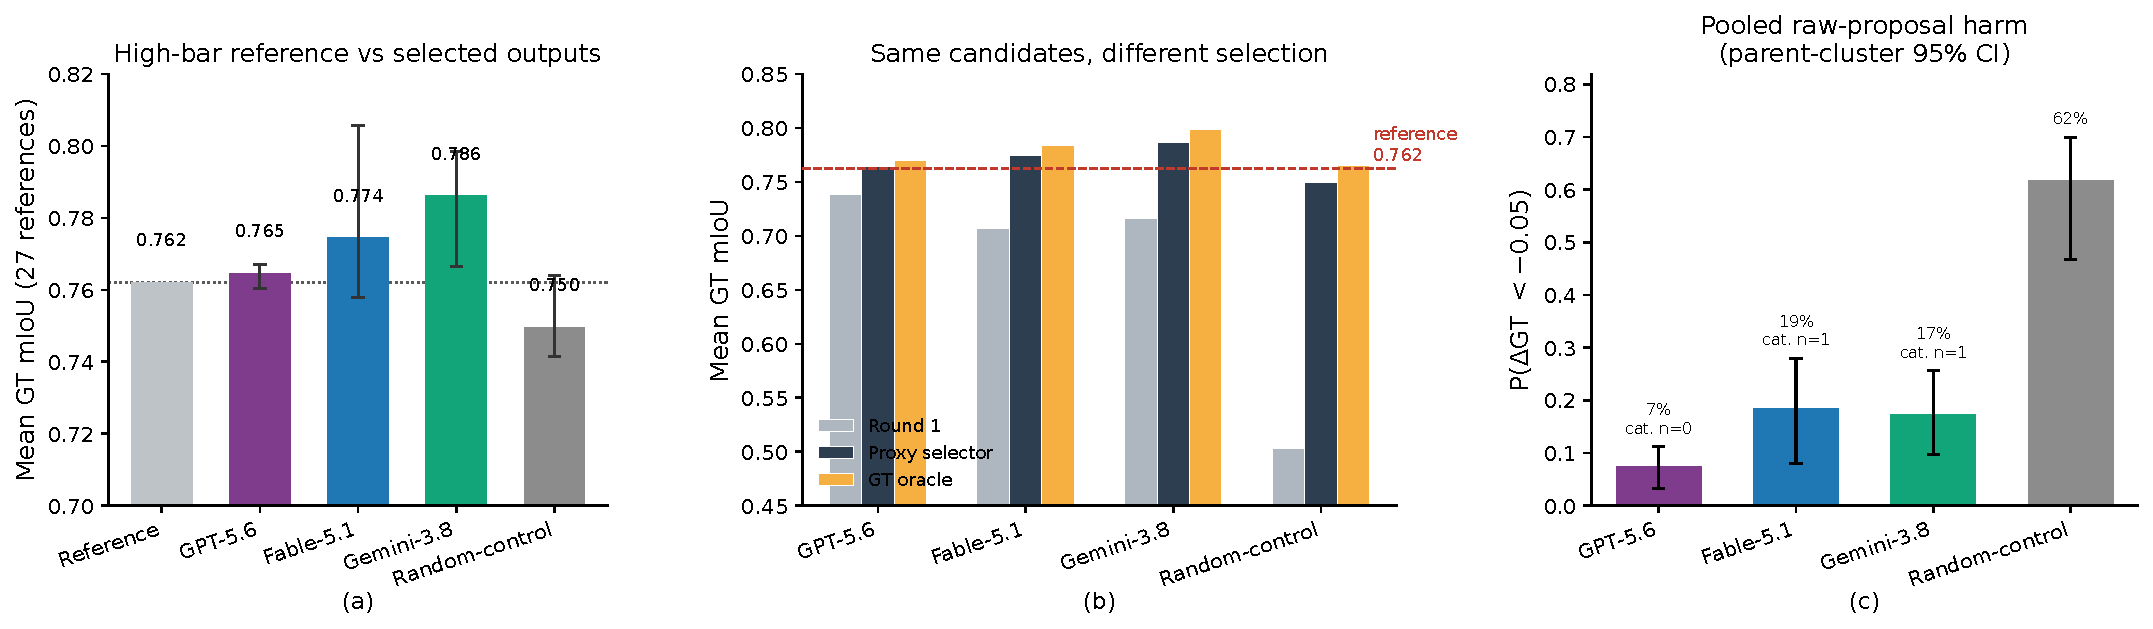
\includegraphics[width=\textwidth]{figs/refinement_results.pdf}
\caption{\textbf{Proxy-guided self-refinement against family-specific references.}
(a)~Selected mean GT mIoU for the shared reference start and four proposal arms on all 27 held-out cases (error bars: parent-tunnel bootstrap 95\% CI on the paired gain).
(b)~Counterfactual selection policies on the same candidates.
(c)~Proposal safety: share of proposals with $\Delta$mIoU $<-0.05$ (annotation: population std of proposal $\Delta$).}
\label{fig:self_refinement_results}
\end{figure*}

\hl{The references set a high bar: mean GT mIoU $0.762$, with 10 of 27 already scoring above $0.7$.}
\hl{After proxy-guided self-refinement, the final outputs exceed $0.7$ in 22/27 (Fable-5.1), 24/27 (Gemini-3.8), and 21/27 (GPT-5.6), with mean selected mIoU $0.774$, $0.782$, and $0.765$, respectively (Table~\ref{tab:arm-compare} and Table~\ref{tab:panel-audit}; Fig.~\ref{fig:self_refinement_results}).} 

\begin{table*}[t]
\caption{Self-refinement on all 27 held-out family-specific references. Selected means use the shared proxy selector with a retention margin: a candidate replaces the retained output only if its proxy score exceeds the retained score by more than $0.01$. Bootstrap CIs are parent-tunnel (100{,}000 resamples).}\label{tab:arm-compare}
{\small
\begin{tabular*}{\textwidth}{@{\extracolsep{\fill}} l c c c c c @{}}
\toprule
Arm & Selected mean & Mean $\Delta$ & 95\% CI & Up/same/down & Worst $\Delta$ \\
\midrule
Reference start & 0.762 & -- & -- & -- & -- \\
Fable-5.1 & 0.774 & $+0.012$ & $[-0.004,\,0.044]$ & 6/15/6 & $-0.143$ \\
Gemini-3.8 & 0.782 & $+0.020$ & $[0.004,\,0.031]$ & 6/12/9 & $-0.185$ \\
GPT-5.6 & 0.765 & $+0.003$ & $[-0.002,\,0.005]$ & 5/20/2 & $-0.013$ \\
Random search & 0.750 & $-0.012$ & $[-0.021,\,0.002]$ & 3/19/5 & $-0.115$ \\
\bottomrule
\end{tabular*}}
\end{table*}

\hl{ Fig.~\ref{fig:self_refinement_results}b separates what the proxy contributes from what the proposer contributes. Accepting every first proposal blindly would have cut the random arm from $0.762$ to $0.503$; the selection rule recovers this to $0.750$, so the proxy does most of the protective work for an uninformed proposer. For the LLM arms the oracle ceiling is higher ($0.770$--$0.794$) and the proxy selector recovers most of it. The proxy therefore fixes the floor; the proposer fixes the ceiling.}



\subsection{Error analysis: residual rotation}
\label{sec:error-analysis}

\begin{figure*}[t]
  \centering
  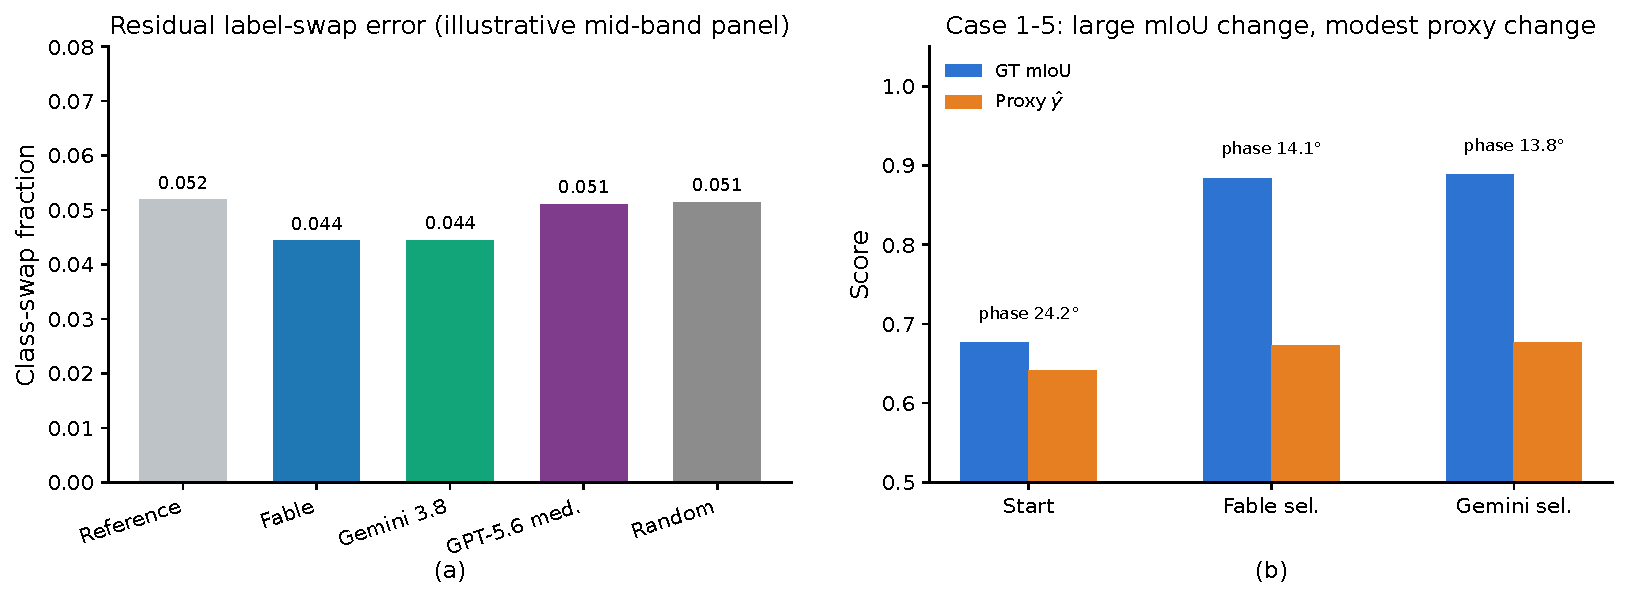
\includegraphics[width=\textwidth]{figs/error_rotation.pdf}
\caption{\textbf{Rotation-related residual error.}
(a)~\hl{Point-level error composition (correct, missed, spurious, swapped) for the reference start and each arm's selected outputs.}
(b)~Case 1-5: large offline mIoU and phase-incoherence changes accompany only modest movement of the four-feature proxy score.}
\label{fig:error_rotation}
\end{figure*}

\hl{Where does the missing precision go? Fig.~\ref{fig:error_rotation}a decomposes point errors: after selection, missed and spurious points barely move, and the arms that gain (Fable-5.1, Gemini-3.8) do so mainly by reducing swapped labels, from $4.0\%$ to about $3\%$. Swaps are the error the proxy sees least well. Case 1-5 shows why (Fig.~\ref{fig:error_rotation}b): Fable and Gemini selections lift GT mIoU from $0.676$ to about $0.88$ and cut phase incoherence from $24^{\circ}$ to $14^{\circ}$, yet the proxy score moves only from $0.641$ to the mid-$0.67$ range. A cyclic relabelling of a whole ring leaves coverage, depth completeness, ring count, and joint--boundary agreement almost unchanged, because every block is still bounded by a detected joint; only its identity is wrong. The four features were chosen for transfer, and phase incoherence, the one candidate that measures this, was not among those that transferred. The largest single losses in Table~\ref{tab:arm-compare} (Fable-5.1 on 3-6, Gemini-3.8 on 2-5) are of the same kind: the proxy rose while GT fell. Rotation-aware evidence is therefore the next feature to add, not a result shown here.}

\begin{table*}[t]
\caption{Positioning Proxy4Tun against representative tunnel-segmentation paradigms. The comparison concerns setup cost and deployment capability as well as accuracy. mIoU figures are \emph{not} measured under comparable settings: supervised and expert-tuned figures are taken from prior work under their original protocols, whereas Proxy4Tun figures are from this study (27 held-out family-specific references).}\label{tab:sota}
\begin{tabular*}{\textwidth}{@{\extracolsep{\fill}} l c c c l @{}}
\toprule
Method & \begin{tabular}[t]{@{}c@{}}Deep learning\\training\end{tabular} & \begin{tabular}[t]{@{}c@{}}Per-case\\tuning\end{tabular} & \begin{tabular}[t]{@{}c@{}}Deployment-label-free\\quality signal\end{tabular} & mIoU (setting) \\
\midrule
LiningNet/SparseUNet/SCF-Net/FA-ResNet & \checkmark & -- & -- & 0.83--0.90 \\
SAM4Tun & -- & Expert & -- & above 0.90 \\
\textbf{Proxy4Tun} (four-feature + LLM) & -- & \textbf{Auto} & \checkmark & \textbf{0.765--0.782} \\
\bottomrule
\end{tabular*}
\end{table*}


% ══════════════════════════════════════════════════════════════════════════
\section{Discussion}\label{sec:discussion}
% ══════════════════════════════════════════════════════════════════════════

\hl{The results answer the research question of Section~\ref{sec:intro} in two parts. Intermediate measurements do carry accuracy information that survives transfer to unseen scans and, less evenly, to unseen families. Guiding self-refinement with that information works only in combination: the proxy prevents an already-good configuration from being spoiled, while whether anything better is found depends on the proposer.}

\subsection{Key findings}

\hl{\textbf{Fewer features transfer better.} The design principle of Section~\ref{sec:methods} was to select for transfer, not fit, and the ablation bears this out: adding six measurements to the compact four lowered LOFO $\rho$ from $0.809$ to $0.686$. With 120 runs from three scans, a proxy that explains its own calibration set is not the goal; one that still orders runs on a family it has not seen is. The cost is coverage: the discarded features include the one sensitive to ring rotation.}

\hl{\textbf{The selection rule is a floor, not a search strategy.} The random arm makes this explicit. Its proposals were disastrous on average, its oracle ceiling was barely above the start, and the selection rule still held the mean within $0.012$ of the reference. Read together with the LLM arms, whose ceilings and selected means are both higher, the selector's contribution is to make bounded search safe enough to try; the gain comes from proposals that respond to pipeline evidence. This is the attribution the random control was designed to provide (Section~\ref{sec:agent-design}).}

\hl{\textbf{What deployment would look like.} Each pipeline release still needs one expert reference per family and one calibration pass. From then on the frozen proxy supplies a label-free score, a fixed threshold separates constructed failures from references, and three bounded attempts cost roughly 15 GPU-minutes. Self-refinement is assisted, auditable reconfiguration against a strong engineering baseline, not autonomous inspection.}

\subsection{Comparison with state-of-the-art}\label{sec:positioning}

Comparisons here concern operating points, not accuracy leaderboards (Table~\ref{tab:sota}). Supervised 3D models on Seg2Tunnel report strong in-distribution accuracy~\cite{lin2024seg2tunnel} but require per-point labels and provide no deployment-time accept/refine/flag gate. Expert-tuned SAM4Tun reaches high accuracy on curated rings~\cite{ye2025sam4tun}, but a fixed configuration emits no signal when it degrades. Relative to that static pipeline, Proxy4Tun adds an explicit quality signal and a bounded self-refinement loop. The only directly comparable contrast in this study is LLM-plus-proxy versus random-plus-proxy under the shared reference starts and \hl{selection rule. The mIoU gap to expert-tuned SAM4Tun in Table~\ref{tab:sota} is therefore not a like-for-like deficit: those figures come from curated rings with per-case expert tuning, whereas the Proxy4Tun figures are 27 unseen subsets with three automated attempts each.}

\subsection{Limitations}\label{sec:limitations}

\hl{Four limitations bound the claims. First, the evidence base is narrow: 120 calibration runs come from three scans, and the 27 held-out subsets share tunnels and families with them. Transfer is shown to unseen scans within this collection, not to new projects or lining geometries, and the weak continuous-family LOFO result ($\rho=0.49$) shows that even within-collection transfer is uneven. Second, the proxy is blind to rotation: the four features chosen for transfer do not register whole-ring relabelling, so proxy gains do not reliably track GT gains, and the two largest LLM losses passed the selection rule for exactly this reason. Third, the degradations are constructed and the panel is small: the test says nothing about false-alarm rates on naturally failed runs, and with five parent tunnels the bootstrap intervals for Fable-5.1 and GPT-5.6 include zero, so their gains are descriptive. Fourth, the loop is one expert reference and three attempts; nothing here shows sustained improvement over longer horizons or without a reference to start from.}


% ══════════════════════════════════════════════════════════════════════════
\section{Conclusions}\label{sec:conclusions}
% ══════════════════════════════════════════════════════════════════════════

\hl{This paper asked whether intermediate tunnel-segmentation measurements can estimate accuracy and guide parameter self-refinement on unseen scans without new GT labels. Proxy4Tun answers with a four-feature Ridge proxy calibrated from 120 runs around one expert reference per lining family, selected for cross-family transfer rather than fit, and frozen before any held-out scan is scored.}

\begin{itemize}
\item \hl{The measurements carry transferable accuracy information. Three structure-coherence features and one preprocessing-quality feature reach Spearman $0.791$ on 54 held-out runs and order every reference above its degraded partner; adding more features hurt transfer.}
\item \hl{The proxy can guide improvement of strong references, but only with an informed proposer. From a $0.762$ baseline, LLM proposals under the selection rule reach $0.765$--$0.782$, while random proposals under the same rule fall to $0.750$ despite the rule blocking most of their damage.}
\item \hl{The roles are separable: the proxy sets the floor by retaining the start, the proposer sets the ceiling, and the proposer's temperament, not the selector, determines the risk of individual losses.}
\end{itemize}

\hl{The principal remaining limit is rotation blindness: the features that transfer do not see whole-ring relabelling, so the proxy can approve a rotated result. Future work should add rotation-aware evidence that transfers as well as the current four, test the loop on naturally degraded runs and on tunnels outside this collection, and examine whether the proxy can guide refinement without an expert reference to start from. Until then, Proxy4Tun is a label-free assessment and assisted-reconfiguration tool, not an autonomous inspector.}

% ══════════════════════════════════════════════════════════════════════════
% Data availability, declarations, etc.
% ══════════════════════════════════════════════════════════════════════════

\section*{Data availability}

The source code, parameter snapshots, exploration-trial tables, and evaluation scripts will be released upon publication. The Seg2Tunnel dataset is publicly available~\cite{lin2024seg2tunnel}.

\section*{Declaration of competing interest}

The authors declare that they have no known competing financial interests or personal relationships that could have appeared to influence the work reported in this paper.

\section*{Declaration of generative AI use}

During this study, LLM agents (Fable-5.1, Gemini-3.8, and GPT-5.6) were evaluated as proposal mechanisms in the self-refinement loop, together with a \hl{random-search control under the same proxy-based selection rule}. LLMs were also used for language editing and for improving manuscript structure. The authors reviewed and edited all content and take full responsibility for the content of the publication.

% ══════════════════════════════════════════════════════════════════════════
% Bibliography
% ══════════════════════════════════════════════════════════════════════════

% Natbib requires a BibTeX style; without it, citations stay as “?”
% NOTE: \balance can cause column-balancing artefacts in the reference list (e.g.,
% lines slipping into the footer area) with this class. Keep it off for the bibliography.
%\balance
\bibliographystyle{model1-num-names}
\bibliography{references}


% ══════════════════════════════════════════════════════════════════════════
% Appendix
% ══════════════════════════════════════════════════════════════════════════

\appendix

\section{Pipeline anchor parameters}\label{app:anchor-parameter}

This appendix summarises the expert-tuned \emph{anchor} parameter profiles used to warm-start the segmentation pipeline for each lining family (staggered, continuous, complex). Table~\ref{tab:anchor-params} lists the fixed stage algorithms and the corresponding family-specific parameter values that define the reference configurations used throughout the study.

\begin{table*}[t]
\caption{Pipeline anchor parameters: expert-tuned, family-specific anchor parameter profiles of the segmentation pipeline.}\label{tab:anchor-params}
\begin{tabular*}{\textwidth}{@{\extracolsep{\fill}} l l p{0.30\textwidth} l @{}}
\toprule
Stage & Parameter & Description & Staggered / Continuous / Complex \\
\midrule
Unfolding & \texttt{diameter} & Cylindrical scale. & 5.5 / 5.9 / 7.5\,m \\
Unfolding & \texttt{slice\_spacing\_factor} & Slice spacing (ring width). & 1.2 / 1.2 / 1.8\,m \\
Unfolding & \texttt{polynomial\_degree} & Centreline fit degree. & 3 / 2 / 2 \\
Unfolding & \texttt{residual\_recentre} & Per-bin frame recentring. & off / on / on \\
\midrule
Denoising & \texttt{mask\_r\_low} & Inner radial gate. & 2.33 / 2.85 / 3.65\,m \\
Denoising & \texttt{mask\_r\_high} & Outer radial gate. & 2.78 / 3.0 / 3.9\,m \\
Denoising & \texttt{y\_step} & Angular bin width. & 0.4 / 0.5 / 0.1\,m \\
Denoising & \texttt{z\_step} & Radial histogram bin width. & 0.005 / 0.001 / 0.001\,m \\
Denoising & \texttt{grad\_threshold} & Outer-edge gradient threshold. & 0.15 / 0.2 / 0.2 \\
Denoising & \texttt{smoothing\_window\_size} & Cutoff-curve smoothing window. & 5 / 3 / 3 \\
Denoising & \texttt{smoothing\_offset} & Post-smoothing cutoff bias. & $-$0.002 / $-$0.003 / $-$0.005\,m \\
Denoising & \texttt{default\_cutoff\_z} & Fallback radial cutoff. & 2.75 / 2.85 / 3.65\,m \\
\midrule
Enhancing & \texttt{upsampling\_stage1} & Stage-1 upsampling spacing. & 0.06 / 0.08 / 0.09\,m \\
Enhancing & \texttt{upsampling\_stage2} & Stage-2 upsampling spacing. & 0.03 / 0.04 / 0.045\,m \\
Enhancing & \texttt{upsampling\_stage3} & Stage-3 upsampling spacing. & 0.015 / 0.02 / 0.0225\,m \\
Enhancing & \texttt{curvature\_threshold} & Panel--joint curvature threshold. & 0.005 / 0.0005 / 0.0005 \\
Enhancing & \texttt{depth\_threshold\_low} & Lower interpolation depth tolerance. & 0.005 / 0.01 / 0.0065\,m \\
Enhancing & \texttt{depth\_threshold\_high} & Upper interpolation depth tolerance. & 0.015 / 0.01 / 0.013\,m \\
Enhancing & \texttt{inter\_radius} & Interpolation neighbour radius. & 0.03 / 0.06 / 0.06\,m \\
Enhancing & \texttt{n\_segment\_start/end} & Interpolated ring-index window. & 0--5 / 2--8 / 5--14 \\
Enhancing & \texttt{ring\_spacing\_factor} & Nominal ring width. & 1.2 / 1.2 / 1.8\,m \\
\midrule
Detecting & \texttt{binary\_threshold} & Depth-map binarisation level. & 125 / 127 / 125 \\
Detecting & \texttt{hough\_thresh\_obliq} & Oblique joint-line vote threshold. & 65 / 30 / 35 \\
Detecting & \texttt{hough\_thresh\_horiz} & Horizontal joint-line vote threshold. & 65 / 30 / 35 \\
Detecting & \texttt{hough\_thresh\_vert} & Ring-boundary vote threshold. & 600 / 1500 / 5000 \\
Detecting & \texttt{minLineLength\_obliq} & Minimum oblique line length. & 100 / 40 /  80\,px \\
Detecting & \texttt{minLineLength\_horiz} & Minimum horizontal line length. & 100 / 50 /  80\,px \\
Detecting & \texttt{maxLineGap\_obliq} & Oblique line-merging gap limit. & 45 / 30 /  60\,px \\
Detecting & \texttt{maxLineGap\_horiz} & Horizontal line-merging gap limit. & 10 / 10 /  15\,px \\
Detecting & \texttt{angle\_range\_oblique} & Oblique-joint angle band. & $\pm$[6, 9] / $\pm$[4, 10] / $\pm$[5, 10]$^{\circ}$ \\
\midrule
Segmenting & \texttt{segment\_per\_ring} & Segments per lining ring. & 6 / 6 / 7 \\
Segmenting & \texttt{segment\_order} & Circumferential segment order. & \begin{tabular}[t]{@{}l@{}}K,B1,A1--A3,B2 /\\K,B2,A3--A1,B1 /\\K,B1,A1--A4,B2\end{tabular} \\
Segmenting & \texttt{segment\_width} & Nominal segment width. & 1200 / 1200 / 1800\,mm \\
Segmenting & \texttt{K\_height} & Key-segment arc height. & 1079.9 / 823.8 / 1227.0\,mm \\
Segmenting & \texttt{AB\_height} & Standard-segment arc height. & 3239.8 / 3346.8 / 3726.9\,mm \\
Segmenting & \texttt{angle} & Oblique K-joint inclination. & 7.52 / 6.12 / 9.8$^{\circ}$ \\
Segmenting & \texttt{processing.y\_bounds} & Valid panorama band. & 3800--13300 / 4500--14000 / 4200--13100\,px \\
\bottomrule
\end{tabular*}
\end{table*}

\section{Bayesian exploration configuration}\label{app:bo-config}

Table~\ref{tab:bo-config} records the frozen design-time exploration settings
used to generate the 120 calibration trials. Accepted trials are exactly
$N_0{=}32$ Sobol $+\,N_{\mathrm{GP}}{=}8$ GP-uncertainty acquisitions per family
(40 valid trials each).

\begin{table*}[t]
\caption{Design-time Bayesian exploration configuration (frozen snapshot).}\label{tab:bo-config}
\begin{tabular*}{\textwidth}{@{\extracolsep{\fill}} l l @{}}
\toprule
Setting & Value \\
\midrule
Target accepted trials / family & $N{=}40$ ($N_0{=}32$ Sobol, $N_{\mathrm{GP}}{=}8$ accepted GP) \\
Sobol & Scrambled QMC in the unit cube \\
GP kernel & Mat\'{e}rn $\nu{=}2.5$ $+$ white noise; \texttt{normalize\_y=True} \\
Length-scale bounds & $(10^{-2},10^{2})$ per dimension; noise $(10^{-6},10^{-1})$ \\
GP optimiser & \texttt{GaussianProcessRegressor}, $n_{\mathrm{restarts\_optimizer}}{=}3$ \\
Acquisition & Maximise predictive std over random candidate pool $\mathcal{P}_{\mathrm{BO}}$ of size $2048$ \\
Failure / top-up rule & Status not ok or required features incomplete $\Rightarrow$ exclude; continue until accepted targets met \\
\bottomrule
\end{tabular*}
\end{table*}

\section{Per-family search-space bounds}\label{app:search-bounds}

This appendix reports the full bounded per-family search spaces $B$ used for Bayesian exploration. Table~\ref{tab:bo-bounds} enumerates every optimised parameter and its allowable range (or discrete set) for each family reference case, defining the constraints enforced during the frozen 120-trial campaign.

\begin{table*}[t]
\caption{Complete per-family search-space bounds $B$ for the frozen 120-trial campaign.}\label{tab:bo-bounds}
{\small
\begin{tabular*}{\textwidth}{@{\extracolsep{\fill}} llp{0.28\textwidth} @{}}
\toprule
Family (case) & Parameter & Bounds \\
\midrule
Staggered (2-1) & \texttt{unfolding.ransac\_threshold} & $[0.8,1.2]$ \\
 & \texttt{unfolding.slice\_spacing\_factor} & $[1.05,1.35]$ \\
 & \texttt{unfolding.polynomial\_degree} & $\{2,3\}$ \\
 & \texttt{unfolding.random\_seed} & $\{0,\ldots,7\}$ \\
 & \texttt{denoising.mask\_r\_low} & $[2.2,2.5]$ \\
 & \texttt{denoising.mask\_r\_high} & $[2.7,2.9]$ \\
 & \texttt{denoising.z\_step} & $[0.001,0.008]$ \\
 & \texttt{denoising.grad\_threshold} & $[0.1,0.25]$ \\
 & \texttt{enhancing.curvature\_threshold} & $[3{\times}10^{-4},8{\times}10^{-3}]$ \\
 & \texttt{enhancing.inter\_radius} & $[0.02,0.08]$ \\
 & \texttt{detecting.binary\_threshold} & $[100,160]$ \\
 & \texttt{detecting.hough\_threshold\_oblique} & $[40,90]$ \\
 & \texttt{detecting.hough\_threshold\_horizontal} & $[40,90]$ \\
 & \texttt{detecting.hough\_threshold\_vertical} & $[400,800]$ \\
 & \texttt{detecting.maxLineGap\_oblique} & $[20,80]$ \\
 & \texttt{sam.y\_bounds\_lower} & $[3600,4400]$ \\
\addlinespace
Continuous (3-1) & \texttt{unfolding.ransac\_threshold} & $[0.8,1.2]$ \\
 & \texttt{unfolding.slice\_spacing\_factor} & $[1.05,1.35]$ \\
 & \texttt{unfolding.polynomial\_degree} & $\{2,3\}$ \\
 & \texttt{unfolding.random\_seed} & $\{0,\ldots,7\}$ \\
 & \texttt{denoising.mask\_r\_low} & $[2.7,3.0]$ \\
 & \texttt{denoising.mask\_r\_high} & $[2.9,3.15]$ \\
 & \texttt{denoising.mask\_theta\_low} & $[1.0,2.5]$ \\
 & \texttt{denoising.mask\_theta\_high} & $[15,19]$ \\
 & \texttt{enhancing.curvature\_threshold} & $[2{\times}10^{-4},2{\times}10^{-3}]$ \\
 & \texttt{detecting.binary\_threshold} & $[100,160]$ \\
 & \texttt{detecting.hough\_threshold\_oblique} & $[20,60]$ \\
 & \texttt{detecting.hough\_threshold\_horizontal} & $[20,60]$ \\
 & \texttt{detecting.hough\_threshold\_vertical} & $[800,2500]$ \\
 & \texttt{detecting.maxLineGap\_oblique} & $[10,60]$ \\
 & \texttt{detecting.pattern\_tolerance} & $[5,20]$ \\
 & \texttt{detecting.uniform\_k\_snap} & $\{\mathrm{off},\mathrm{on}\}$ \\
 & \texttt{sam.segment\_width} & $[1000,1400]$ \\
 & \texttt{sam.K\_height} & $[700,1000]$ \\
 & \texttt{sam.angle} & $[4,9]$ \\
\addlinespace
Complex (5-1) & \texttt{unfolding.ransac\_threshold} & $[0.8,1.2]$ \\
 & \texttt{unfolding.slice\_spacing\_factor} & $[1.6,2.0]$ \\
 & \texttt{unfolding.polynomial\_degree} & $\{2,3\}$ \\
 & \texttt{unfolding.random\_seed} & $\{0,\ldots,7\}$ \\
 & \texttt{denoising.mask\_r\_low} & $[3.5,3.8]$ \\
 & \texttt{denoising.mask\_r\_high} & $[3.75,4.05]$ \\
 & \texttt{enhancing.curvature\_threshold} & $[2{\times}10^{-4},2{\times}10^{-3}]$ \\
 & \texttt{detecting.binary\_threshold} & $[100,160]$ \\
 & \texttt{detecting.hough\_threshold\_oblique} & $[25,70]$ \\
 & \texttt{detecting.hough\_threshold\_horizontal} & $[25,70]$ \\
 & \texttt{detecting.hough\_threshold\_vertical} & $[800,5000]$ \\
 & \texttt{detecting.maxLineGap\_oblique} & $[30,80]$ \\
 & \texttt{detecting.maxLineGap\_horizontal} & $[5,30]$ \\
 & \texttt{detecting.pattern\_tolerance} & $[5,20]$ \\
 & \texttt{sam.segment\_width} & $[1500,2100]$ \\
 & \texttt{sam.K\_height} & $[1000,1500]$ \\
 & \texttt{sam.angle} & $[7,12]$ \\
\bottomrule
\end{tabular*}}
\end{table*}


\section{Tunnel ontology structure}\label{app:ontology}

The reflective agent consults a staged SAM4Tun ontology that encodes pipeline
artifacts, per-stage parameters and quality metrics, failure modes, diagnostic
rules, remediation actions, and inter-stage dependencies. The top-level schema
is summarised below:
We omit the complete YAML and show only the structure plus one representative
stage example.

\begin{lstlisting}[caption={Ontology top-level keys and stage inventory.},label={lst:ontology-structure}]
meta                  # version, domain, coordinate systems
artifacts             # data objects (cloud, depth map, masks, ...)
stages[]              # pipeline stages (unfolding through segmentation):
  stage_1_centreline
  stage_2_denoise
  stage_3_upsample
  stage_4_detection
  stage_5_segmentation
inter_stage_dependencies[]   # upstream cause -> defer local retune
diagnostic_rules[]           # metric patterns -> failure modes
remediation_actions[]        # bounded parameter changes
agent_interface              # {state, diagnosis, proposal}
\end{lstlisting}

\begin{lstlisting}[caption={Example ontology stage: radial denoising failure modes.},label={lst:ontology-example}]
- id: stage_2_denoise
  name: Local density-difference-based denoising
  quality_metrics:
    - id: m_retained_ratio
      healthy: "lining kept; background removed"
    - id: m_bg_leakage
      healthy: "near zero"
  failure_modes:
    - id: f_over_gate
      name: Radial gate too tight
      symptom: "lining removed; holes in later depth map"
    - id: f_under_gate
      name: Radial gate too loose
      symptom: "rails/tube/noise retained downstream"
\end{lstlisting}

\section{Agent prompt structure}\label{app:prompt}

Each reflection round issues a single bounded JSON overlay. The model-facing
prompt is assembled from a fixed skeleton (role, isolation rules, current
state, GT-blind intrinsics, four-feature proxy scores, allowed artifact images,
family parameter bounds, and the required output schema). Listing~\ref{lst:prompt-skeleton}
summarises the skeleton; Listing~\ref{lst:prompt-example} gives one example
proposal. GT mIoU and evaluation directories are never included.

\begin{lstlisting}[caption={Agent-prompt skeleton (per round).},label=lst:prompt-skeleton]
Role: reflective parameter agent for SAM4Tun
Allowed context:
  - family reference priors / warm-start parameters
  - GT-blind intrinsics and four-feature proxy scores
  - stage artifacts (depth map, detections, SAM masks)
  - ontology + bounded family search space
State: subset, family, reference proxy, operating band
Task: diagnose failure mode; propose ONE overlay within bounds
Output JSON keys (required):
  observation, failure_mode, rationale, overlay
\end{lstlisting}

\begin{lstlisting}[caption={Example JSON proposal returned by the agent.},label=lst:prompt-example]
{
  "observation": "Centreline residual is high; unroll shows asymmetric voids.",
  "failure_mode": "f_curve_underfit (under-fit centre curve)",
  "rationale": "Raise polynomial degree and tighten RANSAC before retuning SAM.",
  "overlay": {
    "unfolding": {
      "polynomial_degree": 3,
      "ransac_threshold": 0.9
    }
  }
}
\end{lstlisting}

\section{Random-search control}\label{app:random-search}

\hl{The random-search control} samples sparse overlays to match LLM proposal size. Let $k$ be the number of parameters changed in a round. We draw $k$ from a frozen empirical distribution estimated from an earlier LLM pilot campaign (198 proposals across three LLM arms), then sample $k$ distinct parameters uniformly (without replacement) from the bounded search space and sample each chosen parameter value uniformly within its family-specific bounds. \hl{Unfolding parameters are eligible only when the start's centreline residual exceeds 10\,cm, matching the constraint applied to LLM arms. The overlay is applied to the current retained configuration. The distribution and seed were frozen before any LLM attempt in this study, so the control cannot track the LLM runs it is compared with.}

\begin{hlbox}
\noindent\textbf{Frozen sampling design.} Seed base $20260915$; the generator for case index $i$ and round $r$ is seeded with $20260915+1000\,i+r$. Change-count probabilities $\Pr(k)$, $k=1,\ldots,15$:
\begin{center}
\small
\setlength{\tabcolsep}{3.5pt}
\begin{tabular}{@{}l cccccccc@{}}
\toprule
$k$ & 1 & 2 & 3 & 4 & 5 & 6 & 7 & 8 \\
$\Pr(k)$ & .036 & .005 & .025 & .030 & .046 & .061 & .066 & .051 \\
\midrule
$k$ & 9 & 10 & 11 & 12 & 13 & 14 & 15 & \\
$\Pr(k)$ & .076 & .071 & .157 & .188 & .107 & .076 & .005 & \\
\bottomrule
\end{tabular}
\end{center}
A draw of $k$ larger than the number of eligible parameters is clipped to that number.
\end{hlbox}

\section{Full-panel selection audit}\label{app:poc-selection}

Table~\ref{tab:panel-audit} summarises all 27 held-out family-specific references and the selected offline mIoU under each proposal arm. Starts are the family-specific reference configurations. Selected values follow the shared proxy selector with a retention margin: a candidate replaces the retained output only if its proxy score exceeds the retained score by more than $0.01$.

\begin{table*}[t]
\caption{Merged 27-case panel: reference start and selected GT mIoU by arm.}\label{tab:panel-audit}
{\footnotesize
\begin{tabular*}{\textwidth}{@{\extracolsep{\fill}} l l c cccc @{}}
\toprule
Subset & Family & Start & Fable-5.1 & Gemini-3.8 & GPT-5.6 & Random \\
\midrule
1-1 & staggered & 0.784 & 0.784 & 0.783 & 0.784 & 0.784 \\
1-2 & staggered & 0.809 & 0.809 & 0.809 & 0.809 & 0.809 \\
1-3 & staggered & 0.827 & 0.827 & 0.827 & 0.827 & 0.827 \\
1-4 & staggered & 0.853 & 0.853 & 0.851 & 0.853 & 0.853 \\
1-5 & staggered & 0.676 & 0.884 & 0.888 & 0.676 & 0.676 \\
2-2 & staggered & 0.615 & 0.877 & 0.880 & 0.615 & 0.615 \\
2-3 & staggered & 0.795 & 0.793 & 0.795 & 0.790 & 0.795 \\
2-4 & staggered & 0.835 & 0.807 & 0.835 & 0.835 & 0.835 \\
2-5 & staggered & 0.893 & 0.893 & 0.708 & 0.880 & 0.893 \\
3-2 & continuous & 0.631 & 0.634 & 0.631 & 0.634 & 0.643 \\
3-3 & continuous & 0.808 & 0.808 & 0.807 & 0.808 & 0.808 \\
3-4 & continuous & 0.622 & 0.619 & 0.622 & 0.622 & 0.605 \\
3-5 & continuous & 0.588 & 0.588 & 0.847 & 0.642 & 0.598 \\
3-6 & continuous & 0.836 & 0.693 & 0.821 & 0.837 & 0.836 \\
3-7 & continuous & 0.845 & 0.845 & 0.845 & 0.845 & 0.786 \\
3-8 & continuous & 0.723 & 0.723 & 0.711 & 0.723 & 0.630 \\
3-9 & continuous & 0.820 & 0.820 & 0.820 & 0.820 & 0.820 \\
3-10 & continuous & 0.853 & 0.854 & 0.854 & 0.853 & 0.760 \\
4-1 & complex & 0.741 & 0.741 & 0.741 & 0.741 & 0.741 \\
4-2 & complex & 0.787 & 0.775 & 0.781 & 0.787 & 0.787 \\
4-3 & complex & 0.554 & 0.554 & 0.554 & 0.554 & 0.554 \\
4-4 & complex & 0.784 & 0.807 & 0.807 & 0.808 & 0.669 \\
4-5 & complex & 0.808 & 0.808 & 0.808 & 0.808 & 0.808 \\
5-2 & complex & 0.793 & 0.793 & 0.784 & 0.793 & 0.793 \\
5-3 & complex & 0.762 & 0.761 & 0.762 & 0.762 & 0.762 \\
5-4 & complex & 0.760 & 0.760 & 0.754 & 0.760 & 0.760 \\
5-5 & complex & 0.775 & 0.801 & 0.780 & 0.780 & 0.794 \\
\midrule
Mean & -- & 0.762 & 0.774 & 0.782 & 0.765 & 0.750 \\
\bottomrule
\end{tabular*}}
\end{table*}

\end{document}